\documentclass[10pt,conference]{IEEEtran}

% --- Packages ---
\usepackage{cite}
\usepackage{graphicx}
\graphicspath{{figs/}} % Automatically look for images in the figs/ folder
\usepackage[cmex10]{amsmath}
\interdisplaylinepenalty=2500
\usepackage{amsthm}
\newtheorem{definition}{Definition}
\usepackage{algorithmic}
\usepackage{array}
\usepackage[caption=false,font=footnotesize]{subfig}
\usepackage{url}
\usepackage{color}
\usepackage{multirow}
\usepackage[table]{xcolor}


% --- Custom Hyphenation ---
\hyphenation{op-tical net-works semi-conduc-tor}

\begin{document}

% --- Title & Authors ---
\title{FALIN: Fast and Lightweight Image Networks for Time-Series Classification}

\newif\iffinal
% \finalfalse
\finaltrue
\newcommand{\review}[1]{\textcolor[rgb]{0.19607843137254902, 0.4196078431372549, 0.6588235294117647}{#1}}  % Review needed
\newcommand{\todo}[1]{\textcolor[rgb]{0.6588235294117647, 0.19607843137254902, 0.19607843137254902}{#1}}     % To do
\newcommand{\citethis}[1]{\textcolor[rgb]{0.3686274509803922, 0.5411764705882353, 0.3764705882352941}{#1}} % Cite needed

\iffinal
  \author{
    \IEEEauthorblockN{Olavo Barros}
    \IEEEauthorblockA{Departamento de Informatica\\
    Universidade Federal de Viçosa\\
    Viçosa, Brazil\\
    Email: olavo.barros@ufv.br}
  }
\else
  \author{Sibgrapi paper ID: \cmtid \\ }
\fi

\maketitle

% Add a footnote to link the code
\footnotetext{The code and pre-trained models for FALIN are available at \url{https://github.com/Olavo-B/FALIN}}

% --- Abstract ---
\begin{abstract}
Sequential models for Time-Series Classification (TSC) are highly accurate but computationally prohibitive for edge deployment. We introduce FALIN (\review{Fa}st and \review{L}ightweight \review{I}mage \review{N}etworks), a hardware-aware framework that transforms 1D temporal signals into 2D spatial representations (GAF/STFT). By coupling a lightweight 2D CNN with an XGBoost classification backend, FALIN drastically minimizes physical resource footprints. Evaluations across ten UCR datasets demonstrate an order-of-magnitude reduction in arithmetic overhead (under 25 Million MACs compared to $>$250 Million baselines) while maintaining robust classification accuracy. These results validate FALIN as a highly viable, hardware-friendly solution for real-time TinyML edge AI deployment. The framework's code and pre-trained models are publicly available at \url{https://github.com/Olavo-B/FALIN}
\end{abstract}

\IEEEpeerreviewmaketitle

% --- Sections ---
\section{Introduction}

% This section is critical for the paper's success and is often structured into four or five distinct paragraphs. Ensure you address the following topics:

% \begin{itemize}
%     \item \textbf{Research Context:} Establish a common base of scientific understanding. Write accessibly, avoid overly niche jargon early on, and define your acronyms. 
%     \item \textbf{Research Motivation:} Introduce the relevant literature (with citations). Answer the reader's question: ``What is missing in the state of the art?'' This should culminate in a clear research question or highlight a gap in current knowledge.
%     \item \textbf{Main Objective:} Describe how you answer the question or solve the problem. State your proposal and its novelty clearly, outlining your advantages over existing methods.
%     \item \textbf{Paper Organization:} Provide a roadmap for the reader. (e.g., ``The paper is organized as follows. Section \ref{sec:background} presents the literature overview. The methodology is detailed in Section \ref{sec:proposal}. Section \ref{sec:results} presents the validation results, and conclusions are drawn in Section \ref{sec:conclusions}.'')
% \end{itemize}

% Over the past decade, Time Series Classification (TSC) has become a fundamental task across a multitude of domains, ranging from healthcare monitoring and anomaly detection in industrial IoT, to financial forecasting and cognitive radio networks. The ubiquitous nature of temporal data has driven a surge in research aimed at developing robust and accurate classification models. While traditional machine learning algorithms heavily rely on domain-specific feature engineering, deep learning approaches have revolutionized the field by automatically extracting complex representations from raw data.


% Research Context: Temporal data, or time series data, is prevalent in various domains such as healthcare, finance, and industrial monitoring. The sequential nature of this data introduces unique challenges for classification tasks, necessitating specialized approaches that can effectively capture temporal dependencies.


Over the past decade, Time Series Classification (TSC) has become a fundamental task across a multitude of domains, ranging from healthcare monitoring and anomaly detection in industrial Internet of Things (IoT), to financial forecasting \cite{fawaz2019deep}. While traditional machine learning algorithms heavily rely on domain-specific feature engineering, deep learning approaches have revolutionized the field by automatically extracting complex representations from raw data \cite{karim2018lstm}. However, time series data, characterized by its sequential nature and temporal dependencies, presents unique challenges for classification tasks. Figure \ref{fig:eg_wafer} illustrates representative samples from the Wafer dataset \cite{olszewski2001generalized}. Each sample consists of a univariate time series, where every feature corresponds to a measurement acquired at a specific timestamp. 

\begin{figure}[h]
  \centering
  \includegraphics[width=0.40\textwidth]{imgs/eg_wafer_dataset.png}
  \caption{Examples of time-series samples from the Wafer dataset \cite{olszewski2001generalized}. Each point represents a measurement collected at a specific timestamp.}
  \label{fig:eg_wafer}
\end{figure}


Standard sequential models, such as Recurrent Neural Networks (RNNs) and Long Short-Term Memory (LSTMs), have been widely adopted to capture these dependencies. Despite their accuracy, these models require significant computational resources, heavily relying on continuous memory accesses and complex state updates \cite{fawaz2019deep}. This poses a severe limitation for real-time inference on edge devices, where power consumption, memory, and physical hardware are strictly constrained, and transmitting data to the cloud incurs prohibitive bandwidth and latency costs \cite{shi2016edge}.

To address these limitations, mapping temporal dependencies into geometric structures has emerged as a highly effective alternative to pure sequential processing \cite{molina2025gramian,ting2021implementation}. By applying the Short-Time Fourier Transform (STFT) or Gramian Angular Fields (GAF), 1D temporal signals can be converted into 2D matrices (e.g., spectrograms), condensing complex temporal variations into a static spatial arrangement. While this transformation enables the application of highly efficient 2D Convolutional Neural Networks (CNNs), standard CNN architectures are often overly parameterized for the physical constraints of embedded systems \cite{sandler2018mobilenetv2,tan2019efficientnet, shen2025efficient}. Therefore, a hardware-aware approach is necessary to fully exploit this 1D-to-2D mapping in Edge/IoT environments without suffering from excessive memory overhead.

To address the intersection of temporal data classification and edge computing, this paper presents FALIN, an FPGA Accelerator for Lightweight Image Networks using Transformed Temporal Data. It proposes an initial software implementation of a convolutional neural network (CNN) that dynamically encodes one-dimensional temporal sequences into two-dimensional image representations. This transformation enables the use of lightweight image-based architectures for temporal classification tasks, using the efficiency and parallelism of convolutional operations. The proposed approach focuses on the trade-off between classification accuracy, model complexity, and hardware resource utilization, while also providing a comparison against conventional temporal models designed specifically for sequential data processing.

The main contributions of this work are summarized as follows:

\begin{itemize}
    \item \textbf{Data Transformation:} Propose a methodology to encode 1D time-series into 2D images (STFT/GAF), enabling discriminative feature extraction via lightweight CNNs.
    \item \textbf{Hybrid Classifier:} Replace conventional MLP heads with XGBoost-based classifiers to minimize MAC operations while maintaining high classification accuracy.
    \item \textbf{Performance Evaluation:} Implement and evaluate the framework in PyTorch, assessing the trade-offs between accuracy and computational cost across UCR datasets.
    \item \textbf{Benchmarking:} Compare the proposed approach against state-of-the-art temporal and hybrid models, demonstrating superior computational efficiency.
    \item \textbf{TinyML Foundations:} Establish optimized network architectures and strategies to maximize accuracy-to-MAC efficiency for future FPGA-based edge computing deployment.
\end{itemize}


The remainder of this paper is organized as follows. Section \ref{sec:related} presents the related work regarding temporal data transformations and hardware accelerators. The methodology, detailing the GAF data transformation and the proposed FALIN architecture, is described in Section \ref{sec:falin}. Section \ref{sec:results} presents the validation results and hardware synthesis, and conclusions are drawn in Section \ref{sec:conclusions}.

\section{Related Work}
\label{sec:related}

Traditional TSC methods rely on sequential models that directly process temporal dependencies. Architectures such as LSTM networks and hybrid approaches like LSTM-FCN have demonstrated strong performance across benchmark datasets by combining recurrent and convolutional feature extraction mechanisms \cite{karim2018lstm}. More recently, convolutional architectures such as FCN, ResNet, and InceptionTime have achieved state-of-the-art results, although often at the cost of increased computational complexity.

An alternative approach consists of transforming one-dimensional temporal signals into two-dimensional image representations. Wang and Oates \cite{wang2015imaging} introduced GAF and Markov Transition Fields (MTF), demonstrating that temporal patterns can be encoded as images and effectively processed by CNN. Similarly, Ting et al. \cite{ting2021implementation} employed STFT spectrograms combined with a 2D CNN for fetal ECG detection, showing that temporal-to-image transformations can achieve high classification accuracy while enabling efficient hardware implementations.

Recent research on edge AI and FPGA acceleration has focused on reducing the computational cost of CNN inference through lightweight architectures and hardware-aware optimizations. Works such as Shen et al. \cite{shen2025efficient} exploit depthwise separable convolutions to decrease resource utilization on low-end FPGAs, while surveys highlight the importance of minimizing parameters, memory accesses, and arithmetic operations for efficient deployment \cite{diaconu2025survey}. However, most image-based TSC approaches still employ conventional neural classification heads. This work investigates the combination of lightweight CNN feature extractors and XGBoost classifiers operating on GAF and STFT representations, aiming to improve the accuracy-to-complexity trade-off while reducing the number of MAC operations.

\section{The FALIN Framework}
\label{sec:falin}

This section details the proposed FALIN framework. Unlike traditional approaches that adapt generic deep learning models to embedded hardware, FALIN establishes a holistic pipeline where the data representation, network topology, and hardware deployment constraints are jointly optimized. The framework operates in two main phases: a 1D-to-2D data transformation that maps temporal dependencies into spatial structures, followed by a hardware-aware asymmetrical convolutional neural network coupled with an optimized classifier backend.

\subsection{Data Transformation}
\label{subsec:data_transformation}

Conventional sequence models, such as LSTM networks \cite{hochreiter1997long} and RNNs \cite{schmidt2019recurrent}, rely on recurrent state updates that impose severe sequential memory access bottlenecks, making them highly inefficient for parallel hardware accelerators like FPGAs. To bypass these constraints, FALIN shifts the computing paradigm from the temporal domain to the spatial domain by converting 1D continuous signals into 2D geometric matrices. This transformation allows the system to exploit the highly parallelized execution patterns of 2D CNNs natively supported by FPGA structural blocks.

FALIN integrates two complementary encoding strategies tailored to different signal characteristics:
\begin{itemize}
    \item \textbf{Short-Time Fourier Transform (STFT):} The 1D temporal signal is segmented using sliding windows and transformed into the frequency domain via the Fast Fourier Transform (FFT). The resulting 2D spectrogram effectively represents the localized time-frequency energy distribution. This approach is highly effective for high-frequency periodic data, such as machinery vibration or electrocardiogram (ECG) waveforms, where spectral features are strongly discriminative.
    \item \textbf{Gramian Angular Field (GAF):} The time series is first normalized to a strict $[-1, 1]$ interval and encoded into a polar coordinate system, where the amplitude represents the angular cosine and the time step represents the radius. By computing the trigonometric sum or difference between all pairs of time steps, a Gramian Angular Summation Field (GASF) or Gramian Angular Difference Field (GADF) matrix is generated. GAF preserves absolute temporal correlations and converts sequential patterns into rich, dense textures that are easily interpretable by spatial filters.
\end{itemize}

By regularizing diverse 1D inputs into standard 2D image matrices, the data transformation front-end provides a uniform data boundary, ensuring hardware scalability without requiring physical reconfiguration for different sequence lengths.



\begin{figure}[h]
    \centering
    \subfloat[STFT Spectrogram]{
        \includegraphics[width=0.20\textwidth]{imgs/dataset_example_image_stft.png}
        \label{fig:stft_representation}
    }
    \hfill
    \subfloat[GAF Matrix]{
        \includegraphics[width=0.20\textwidth]{imgs/dataset_example_image_gaf.png}
        \label{fig:gaf_representation}
    }
    \caption{The FALIN data transformation options for Wafer dataset \cite{olszewski2001generalized}: alternative 2D spatial representations generated from the 1D continuous temporal inputs.}
    \label{fig:data_transformation_comparison}
\end{figure}

Fig.~\ref{fig:data_transformation_comparison} illustrates the data transformation of the FALIN framework, where 1D temporal signals are mapped into alternative 2D spatial representations. As shown in Fig.~\ref{fig:stft_representation}, the spectrogram derived from the STFT highlights the localized time-frequency energy distribution of the continuous signal. Alternatively, Fig.~\ref{fig:gaf_representation} showcases the GAF matrix, which encodes and preserves absolute temporal correlations dense textures. This geometric mapping is essential as it shifts the computational paradigm from temporal sequences to spatial arrangements, enabling structural features to be extracted and processed with high parallel efficiency by the hardware-friendly 2D CNN.

Following the temporal-to-spatial mapping, FALIN performs a crucial hardware-aware resolution normalization to accommodate the strict on-chip memory (BRAM) limits of edge devices. By aggressively resizing all raw, variably sized STFT and GAF outputs into a fixed, low-resolution footprint (e.g., $96 \times 96$ pixels), the framework establishes a deterministic memory access pattern. This spatial standardization allows the FPGA accelerator to process time-series of arbitrary lengths without requiring physical structural reconfiguration. Furthermore, this downsampling quadratically reduces the Multiplier-Accumulator (MAC) operations in subsequent convolutional stages, deliberately trading a marginal loss of fine-grained spatial textures for the optimal computational efficiency required by TinyML constraints. 


\subsection{Architecture}
\label{subsec:architecture}

The neural architecture of FALIN is strictly guided by hardware-aware design principles, focusing on minimizing both the MAC operations and the on-chip memory footprint (BRAMs and registers). To achieve a TinyML-compliant footprint, the proposed 2D CNN is built as a highly compact, three-stage convolutional feature extractor. 

Each processing block applies standard, symmetric $3 \times 3$ convolutional kernels. While maintaining a small spatial footprint, the network carefully limits the channel expansion across its depth (e.g., from 16, to 32, and finally to a 64-dimensional descriptor size). This conservative channel scaling restricts the proliferation of trainable weights and eliminates redundant memory fetch cycles, dramatically lowering the hardware cost while preserving sufficient capacity to capture edges and transition patterns in the transformed STFT or GAF images.

To detail the data flow and feature map transformations, Table~\ref{tab:architecture} presents the layer-by-layer topology of the FALIN CNN. A major architectural bottleneck for deploying CNNs on FPGAs is the rigid input resolution and the parameter explosion associated with standard Fully Connected layers. To resolve this, FALIN integrates an Adaptive Global Average Pooling layer at the end of the final block. This structural optimization ensures spatial invariance, allowing the accelerator to process varying 2D input dimensions without architectural recompilation, while acting as a heavy regularizer to combat overfitting on small-scale tabular datasets.


\begin{table}[htbp]
    \centering
    \caption{FALIN Hardware-Aware Convolutional Architecture}
    \label{tab:architecture}
    \resizebox{0.75\columnwidth}{!}{%
    \begin{tabular}{lcc}
        \hline
        \textbf{Layer / Operation} & \textbf{Ker./Str.} & \textbf{Ch.} \\
        \hline
        \rowcolor{gray!15} Transformed 2D Image & - & 1 \\
        Conv2D + BN + ReLU & $3 \times 3$ / 1 & 16 \\
        \rowcolor{gray!15} MaxPool2D & $2 \times 2$ / 2 & 16 \\
        Conv2D + BN + ReLU & $3 \times 3$ / 1 & 32 \\
        \rowcolor{gray!15} MaxPool2D & $2 \times 2$ / 2 & 32 \\
        Conv2D + BN + ReLU & $3 \times 3$ / 1 & 64 \\
        \rowcolor{gray!15} \textbf{AdaptiveAvgPool2D} & Global / 1 & \textbf{64} \\
        Flatten & - & 64 \\
        \rowcolor{gray!15} Dropout ($p=0.5$) & - & 64 \\
        Linear FC \textit{or} XGBoost & - & Classes \\
        \hline
    \end{tabular}%
    }
\end{table}

Finally, for the decision boundary, the architecture provides a flexible, dual-mode classification backend. For end-to-end hardware inference, it utilizes a lightweight linear classifier regularized by a heavy dropout layer ($p=0.5$). Alternatively, the network can bypass the linear layer entirely, acting solely as a robust feature extractor. In this hybrid mode, the dense descriptor vector is fed into an external XGBoost pipeline. This configuration intent to use robust tree-based ensembles to deliver a robust model accuracy using just Look-Up-Tables, a more abundant resource in low-end FPGAs \cite{https://doi.org/10.1002/cpe.70744, khataei2025treelut}.

\section{Experimental and Results}
\label{sec:results}


\subsection{Used Datasets}
\label{subsec:datasets}

To evaluate the performance of FALIN, we conducted experiments using ten distinct datasets from the UCR Time Series Archive \cite{8894743}. This selection spans a wide range of domains, including medical diagnostics, industrial monitoring, and image recognition, to ensure the framework's versatility. Table~\ref{tab:datasets} summarizes the characteristics of the selected datasets.

\begin{table}[htbp]
    \centering
    \caption{Summary of the Selected UCR Datasets}
    \label{tab:datasets}
    \resizebox{0.85\columnwidth}{!}{%
    \begin{tabular}{lcccc}
        \hline
        \textbf{Dataset} & \textbf{Classes} & \textbf{Samples} & \textbf{Length} & \textbf{Domain} \\
        \hline
        \rowcolor{gray!15} ElectricDevices & 7 & 8926 & 96 & Sensor \\
        StarLightCurves & 3 & 1000 & 1024 & Astronomy \\
        \rowcolor{gray!15} Wafer & 2 & 1000 & 152 & Sensor \\
        ECG5000 & 5 & 500 & 140 & Medical \\
        \rowcolor{gray!15} TwoPatterns & 4 & 1000 & 128 & Synthetic \\
        FordA & 2 & 3601 & 500 & Automotive \\
        \rowcolor{gray!15} FordB & 2 & 3636 & 500 & Automotive \\
        Yoga & 2 & 300 & 426 & Image \\
        \rowcolor{gray!15} Mallat & 8 & 55 & 1024 & Synthetic \\
        FacesUCR & 14 & 200 & 131 & Image \\
        \hline
    \end{tabular}%
    }
\end{table}


\subsection{Training Parameters and Dynamic Heuristics}
\label{subsec:training}

All neural network models and baseline architectures were implemented using the PyTorch framework, leveraging GPU acceleration for the offline training phase. To guarantee strict reproducibility across all experimental runs, deterministic behavior was enforced by locking global random seeds across the Python environment, NumPy operations, and the CUDA backend. The networks were trained for a maximum of 200 epochs using a categorical cross-entropy loss function and a mini-batch size of 64, maintaining an optimal balance between gradient stability and memory footprint.

Given the extreme variance in dataset sizes within the UCR Time Series Archive—ranging from tens to thousands of temporal samples—a static training configuration is highly susceptible to severe overfitting on smaller datasets and suboptimal convergence on larger ones. To address this, the proposed framework employs a dynamic hyperparameter scaling strategy. The initial learning rate ($\eta$) for the Adam optimizer is heuristically determined based on the total number of training samples ($N_s$). It is aggressively regularized to $5 \times 10^{-5}$ for extremely small datasets ($N_s < 200$), adjusted to $1 \times 10^{-4}$ for medium datasets ($200 \le N_s < 1000$), and set to $3 \times 10^{-4}$ for more extensive datasets ($N_s \ge 1000$).

Similarly, to robustly mitigate overfitting while allowing sufficient exploratory iterations, the early stopping mechanism and learning rate scheduler utilize adaptive patience thresholds scaled by the number of mini-batches per epoch ($N_b$). The training process halts automatically if the validation accuracy exhibits no improvement for $P_{stop} = \max(30, \lfloor N_b / 3 \rfloor)$ consecutive epochs. Upon triggering this dynamic early stop, the framework systematically restores the model weights associated with the highest validation performance, ensuring the exported TinyML model is strictly optimal. 

For the hybrid architectures (e.g., FALIN-XGB), the convolutional backbone is frozen post-training to act as a deterministic spatial feature extractor, outputting a compact 128-dimensional descriptor vector. The subsequent XGBoost classifier is then fitted using a multi-class softmax objective function. To balance decision boundary complexity and inference latency, the tree-based backend was configured with a maximum depth of 6, 50 boosting estimators, and a learning rate of $0.1$.

Figure \ref{fig:wafer_metrics_grid} illustrates the training and validation learning curves for the evaluated architectures on the Wafer dataset. As depicted in the loss trajectories, the dynamic early-stopping heuristic successfully intercepts the training process before the onset of severe overfitting, halting execution exactly when validation performance plateaus. 

The custom FALIN architecture demonstrates a convergence profile, even with a high variance in training samples, validating the efficacy of its hardware-aware design and asymmetric kernels in extracting relevant spatial-temporal features from the transformed 2D representations. The MobileNetV2 baseline, while achieving a similar final accuracy, exhibits a stable convergence pattern but with a higher computational cost due to its deeper architecture.

Furthermore, for the hybrid architectures (FALIN-XGB and MobileNet-XGB), these curves represent the end-to-end optimization of the convolutional backbones prior to the weights being frozen for the final decision-tree fitting. Ultimately, the consistent convergence and high validation accuracy across all models confirm a critical hypothesis of this work: the aggressive spatial downsampling to a $96 \times 96$ resolution preserves the essential discriminative features. This allows the system to satisfy the strict memory footprint and Multiplier-Accumulator (MAC) constraints of FPGA edge deployment without sacrificing predictive reliability.

\begin{figure}[htbp]
    % \centering
    
    % --- LINHA 1: FalinCNN ---
    \subfloat[FalinCNN: Accuracy \label{fig:wafer_acc_falincnn}]{
        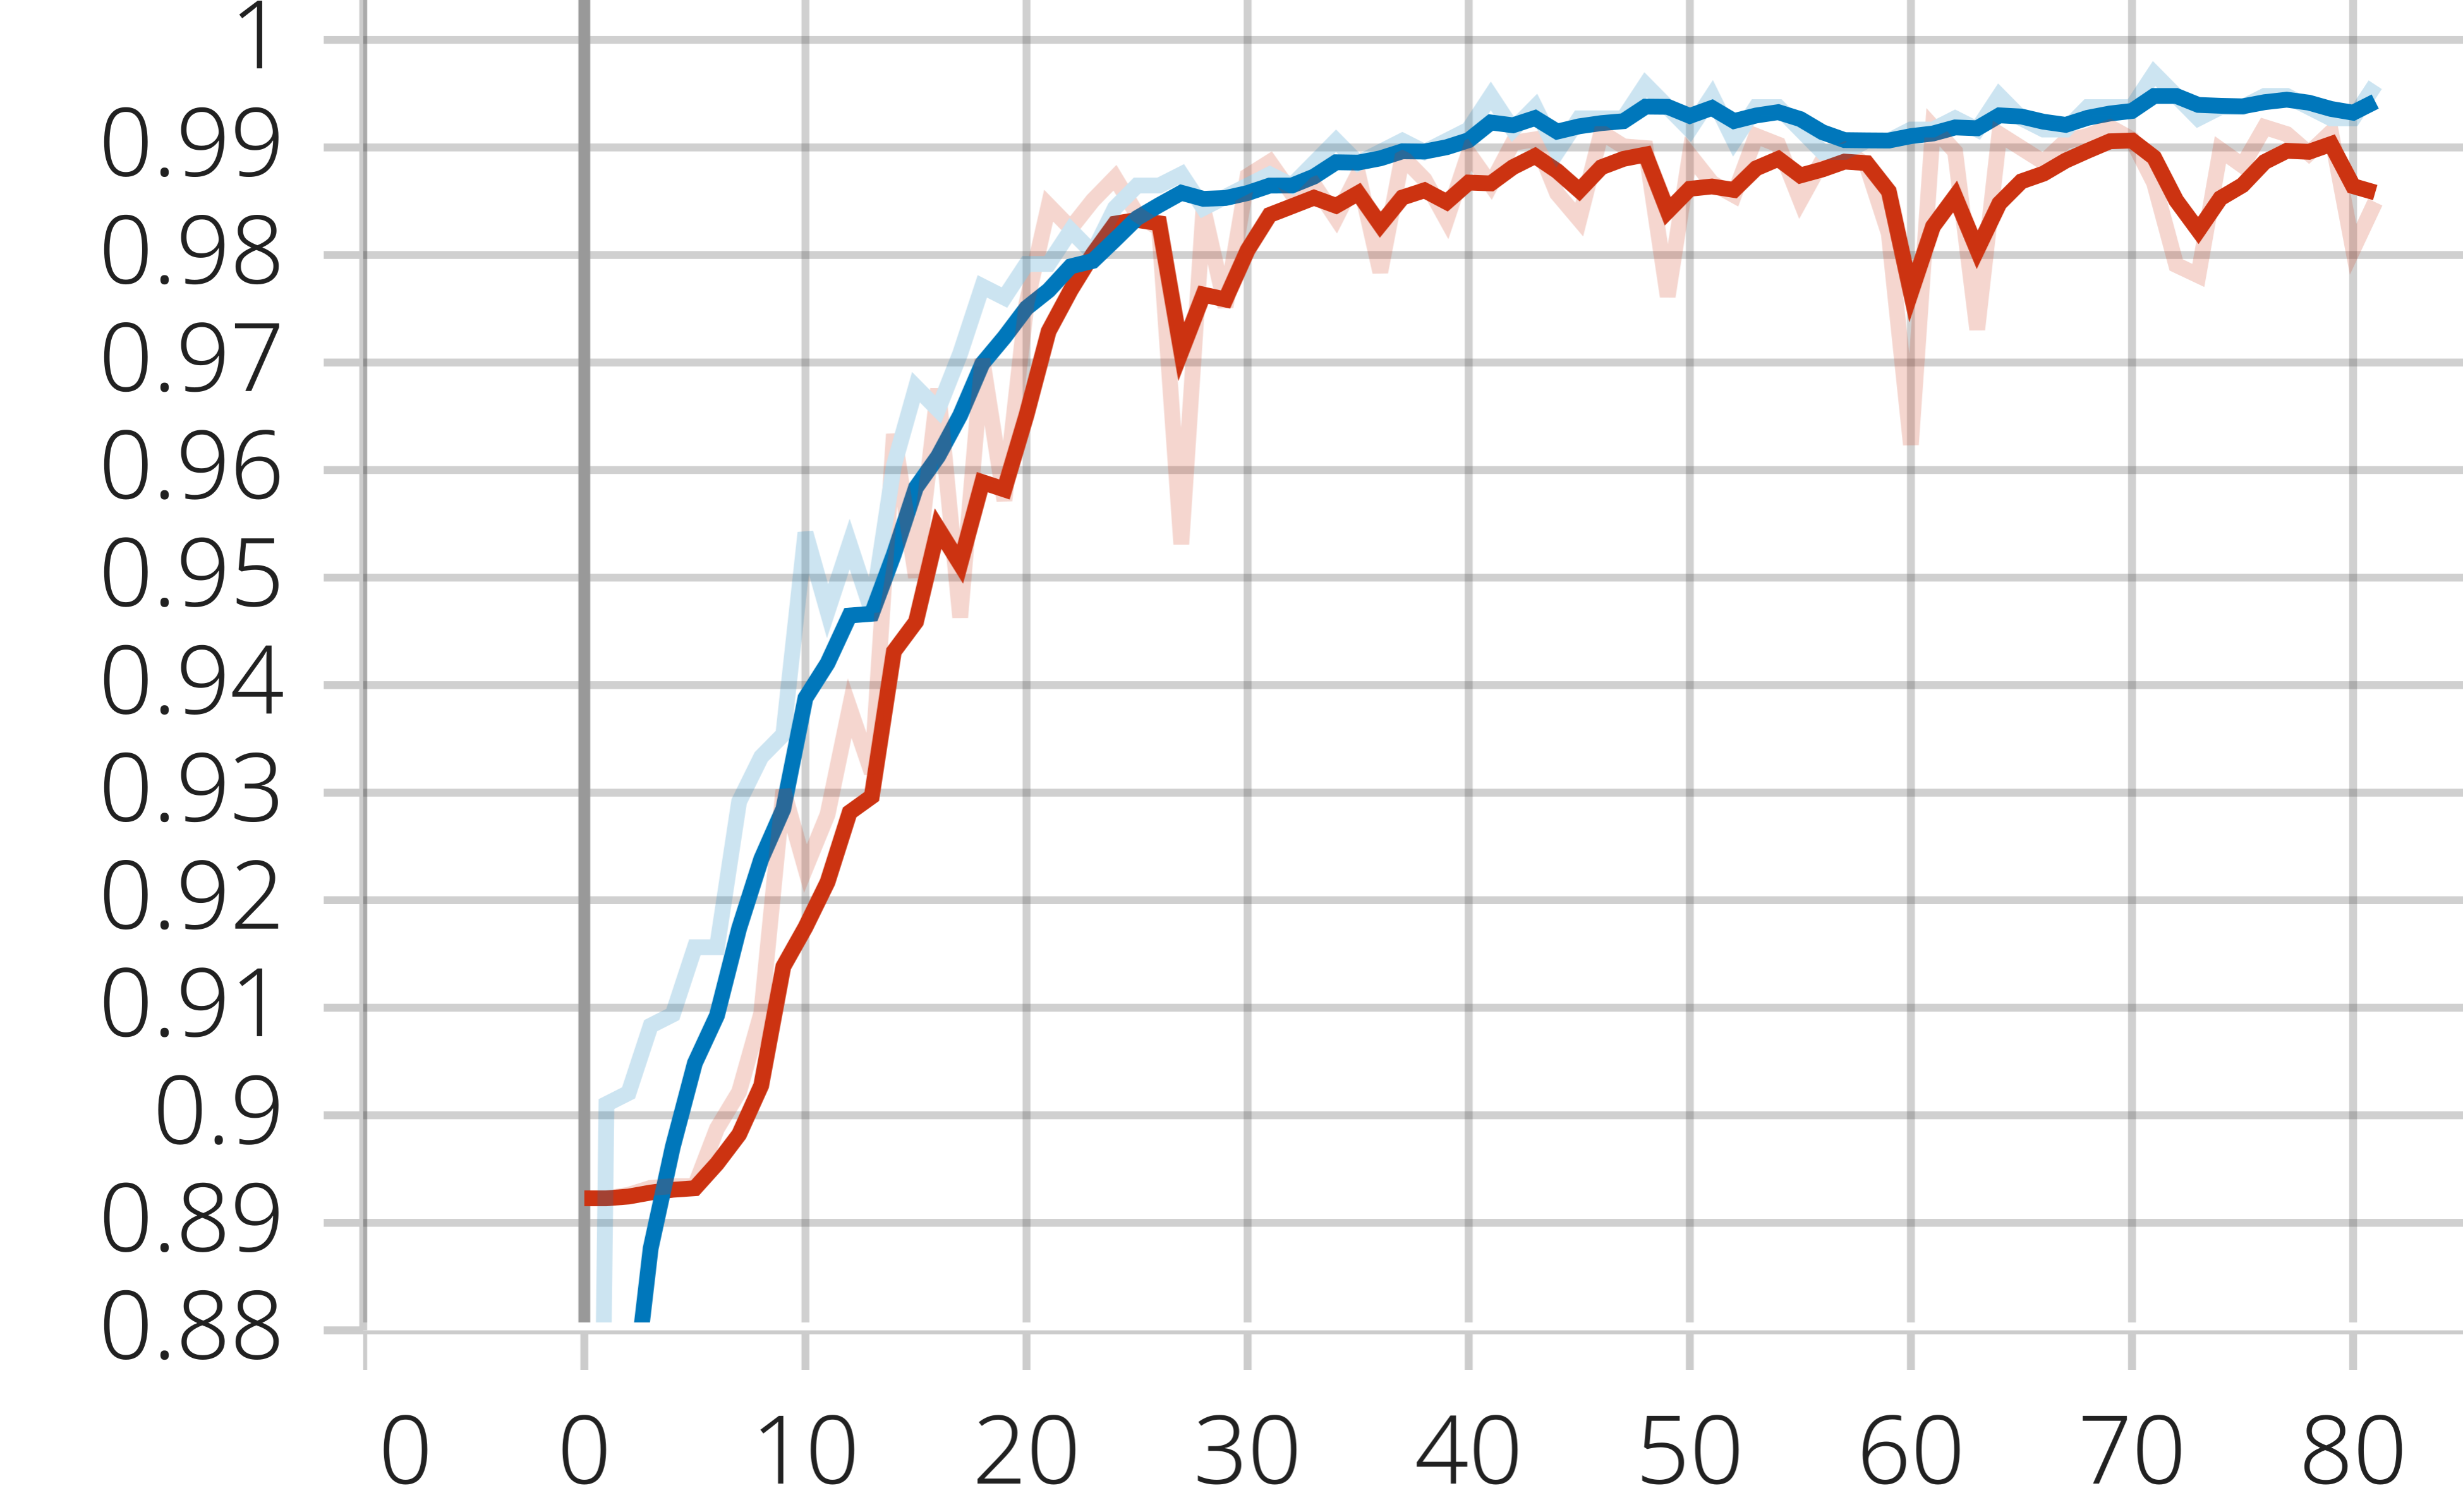
\includegraphics[width=0.24\textwidth]{imgs/Accuracy_falincnn.png}
    }
    % \hfill
    \subfloat[FalinCNN: Loss \label{fig:wafer_loss_falincnn}]{
        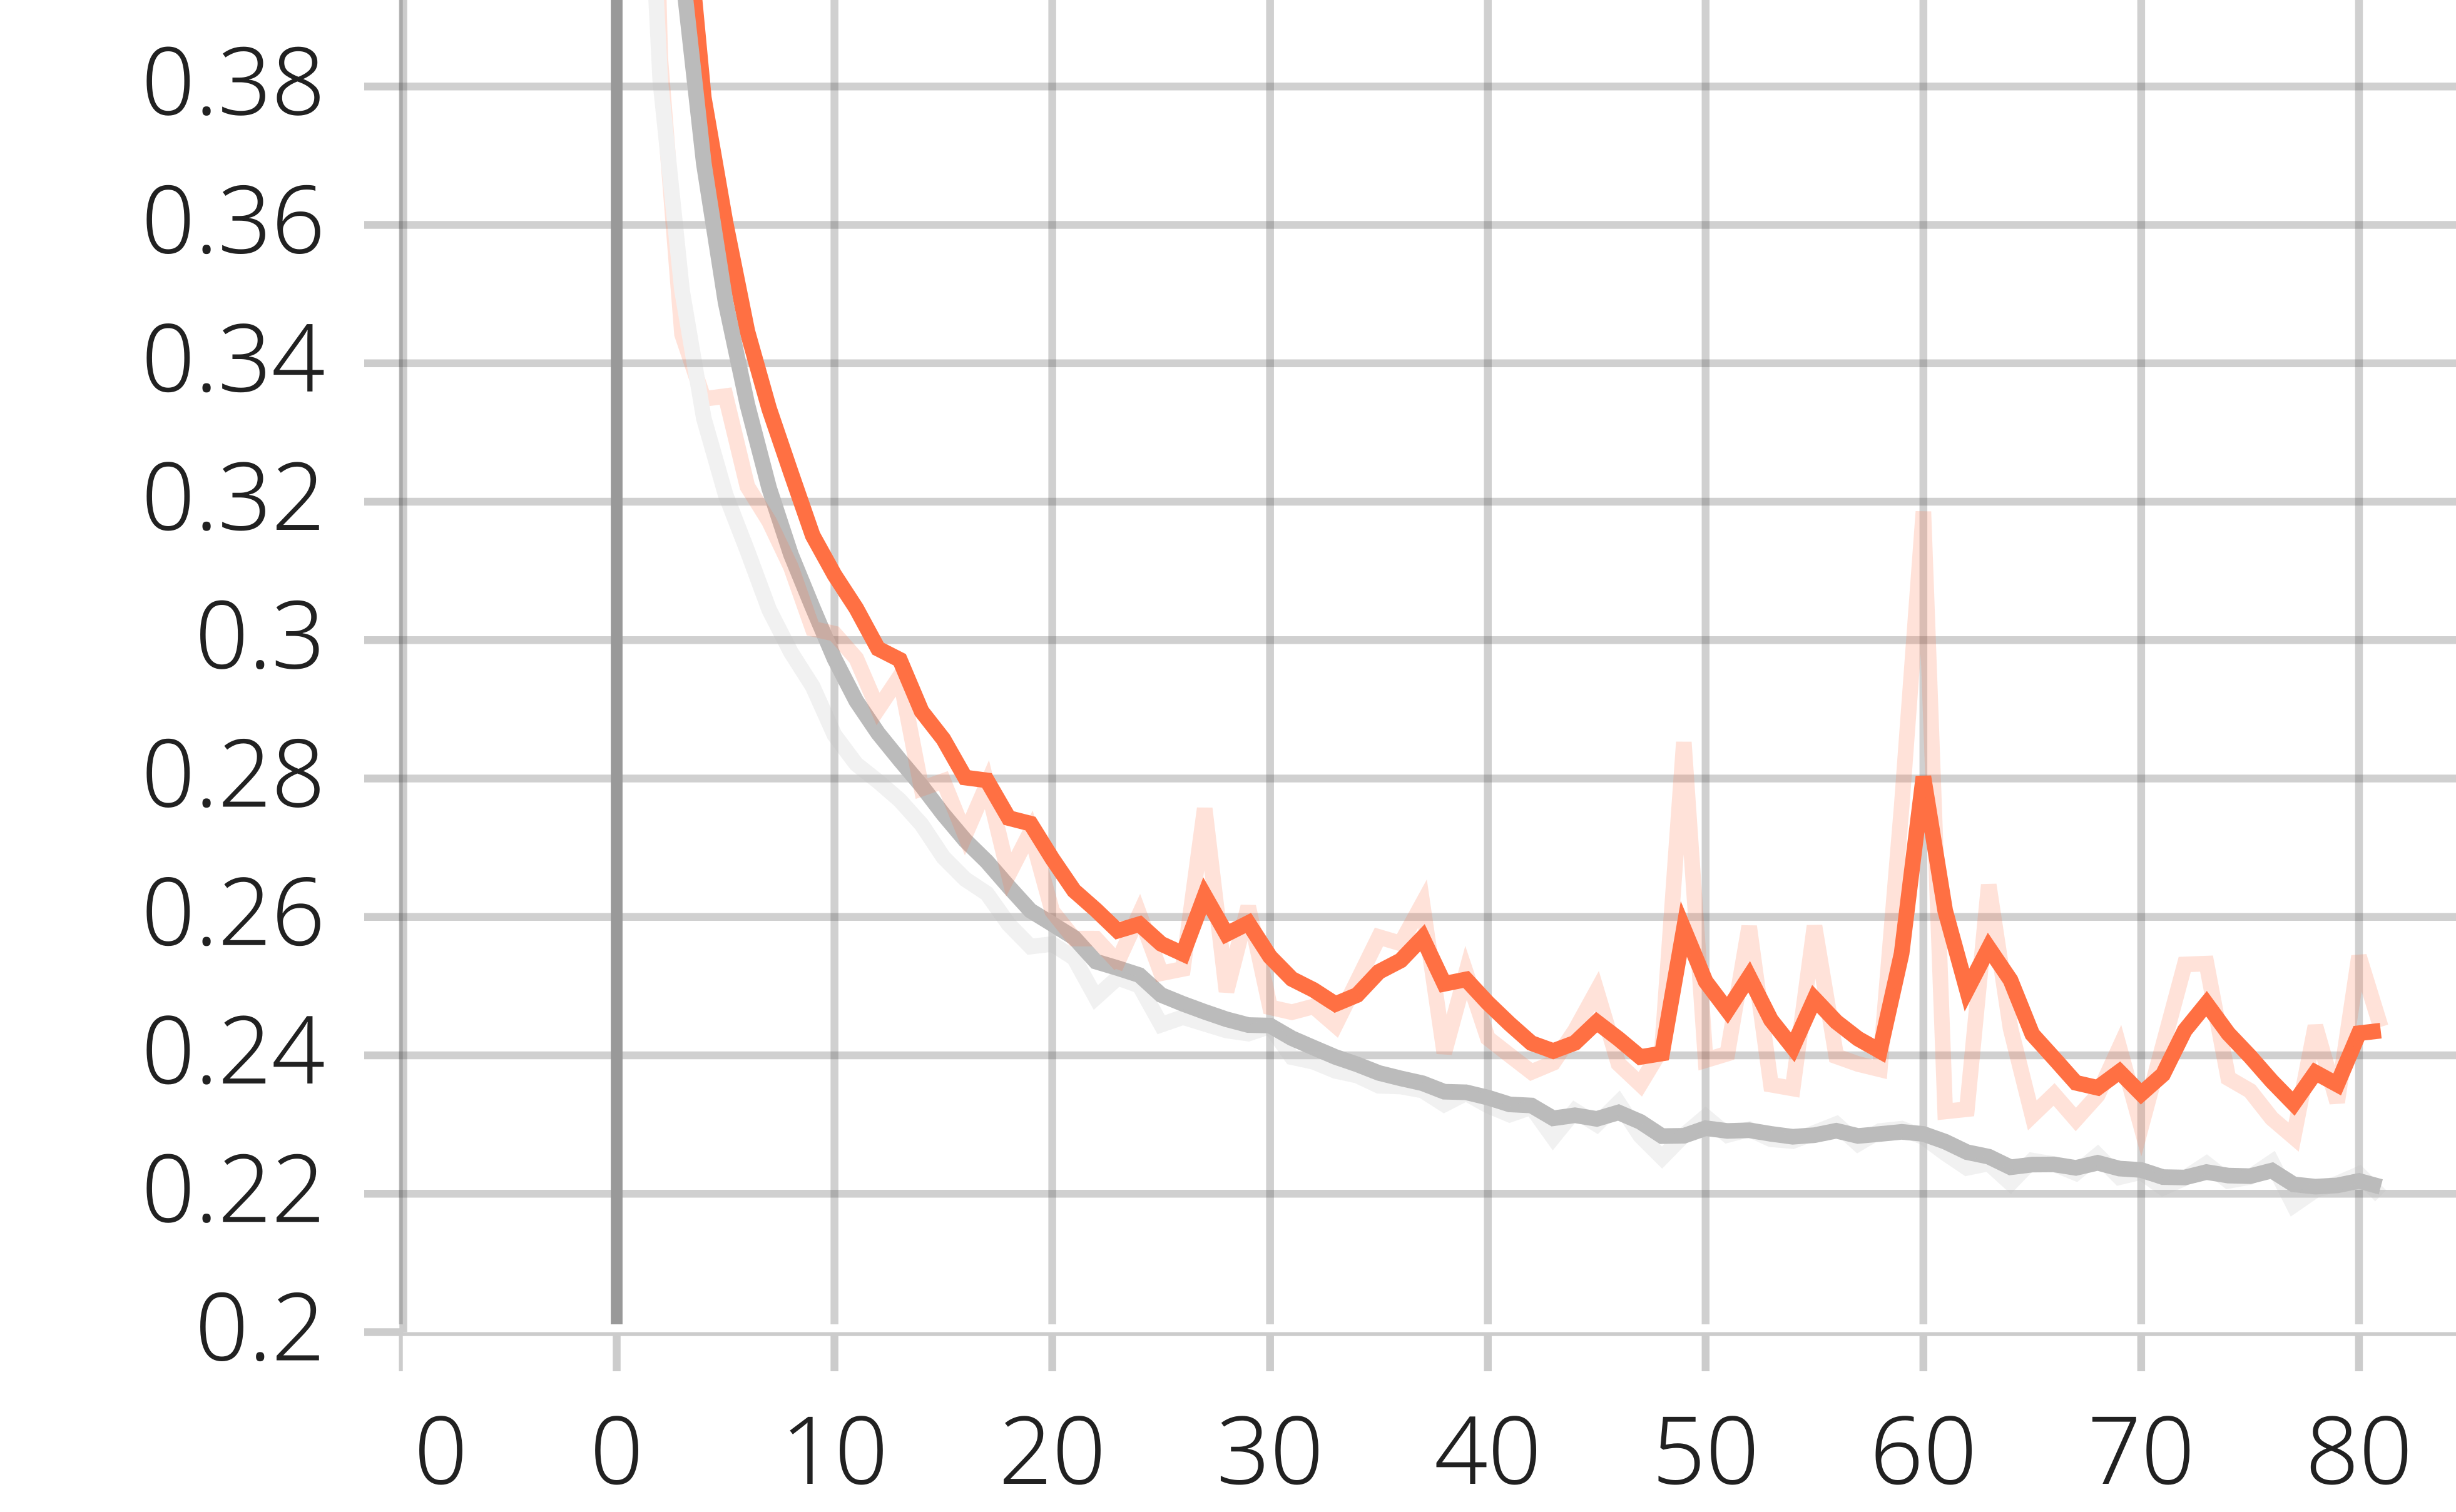
\includegraphics[width=0.24\textwidth]{imgs/Loss_falincnn.png}
    }
    
    \vspace{0.3cm}
    
    % --- LINHA 2: Falin-XGB ---
    \subfloat[FALIN-XGB: Accuracy \label{fig:wafer_acc_falinxgb}]{
        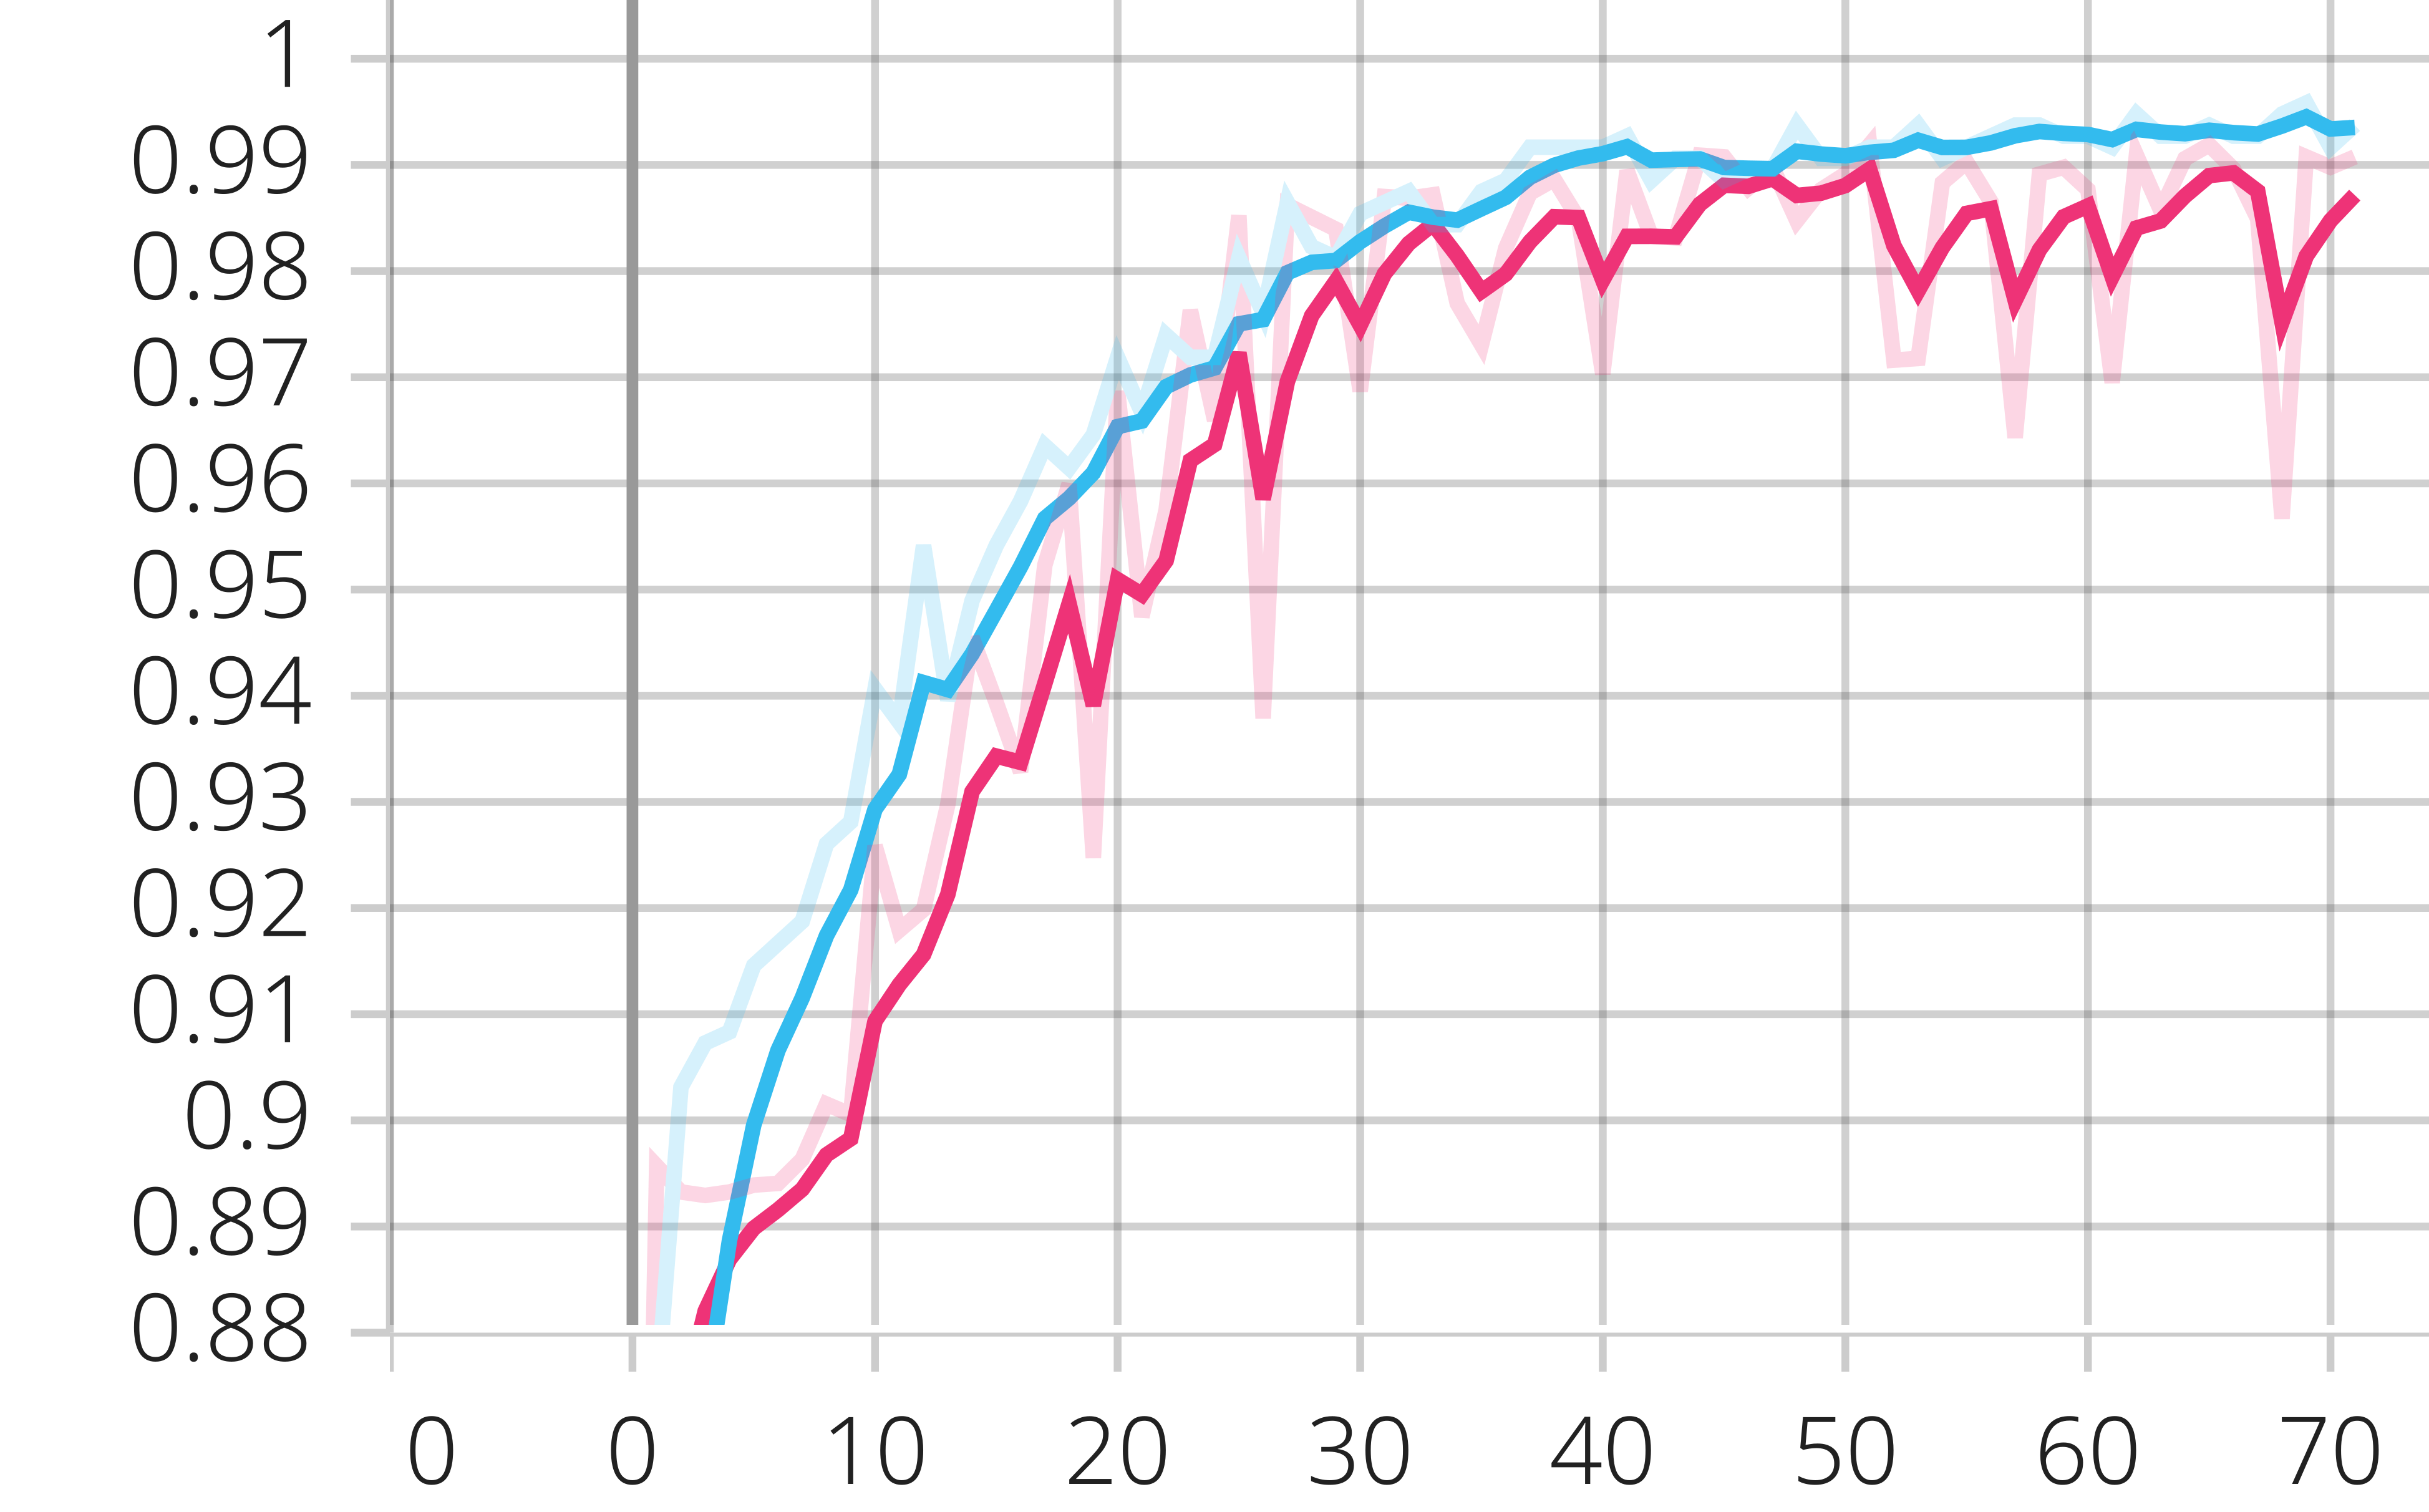
\includegraphics[width=0.24\textwidth]{imgs/Accuracy_falinxgb.png}
    }
    % \hfill
    \subfloat[FALIN-XGB: Loss \label{fig:wafer_loss_falinxgb}]{
        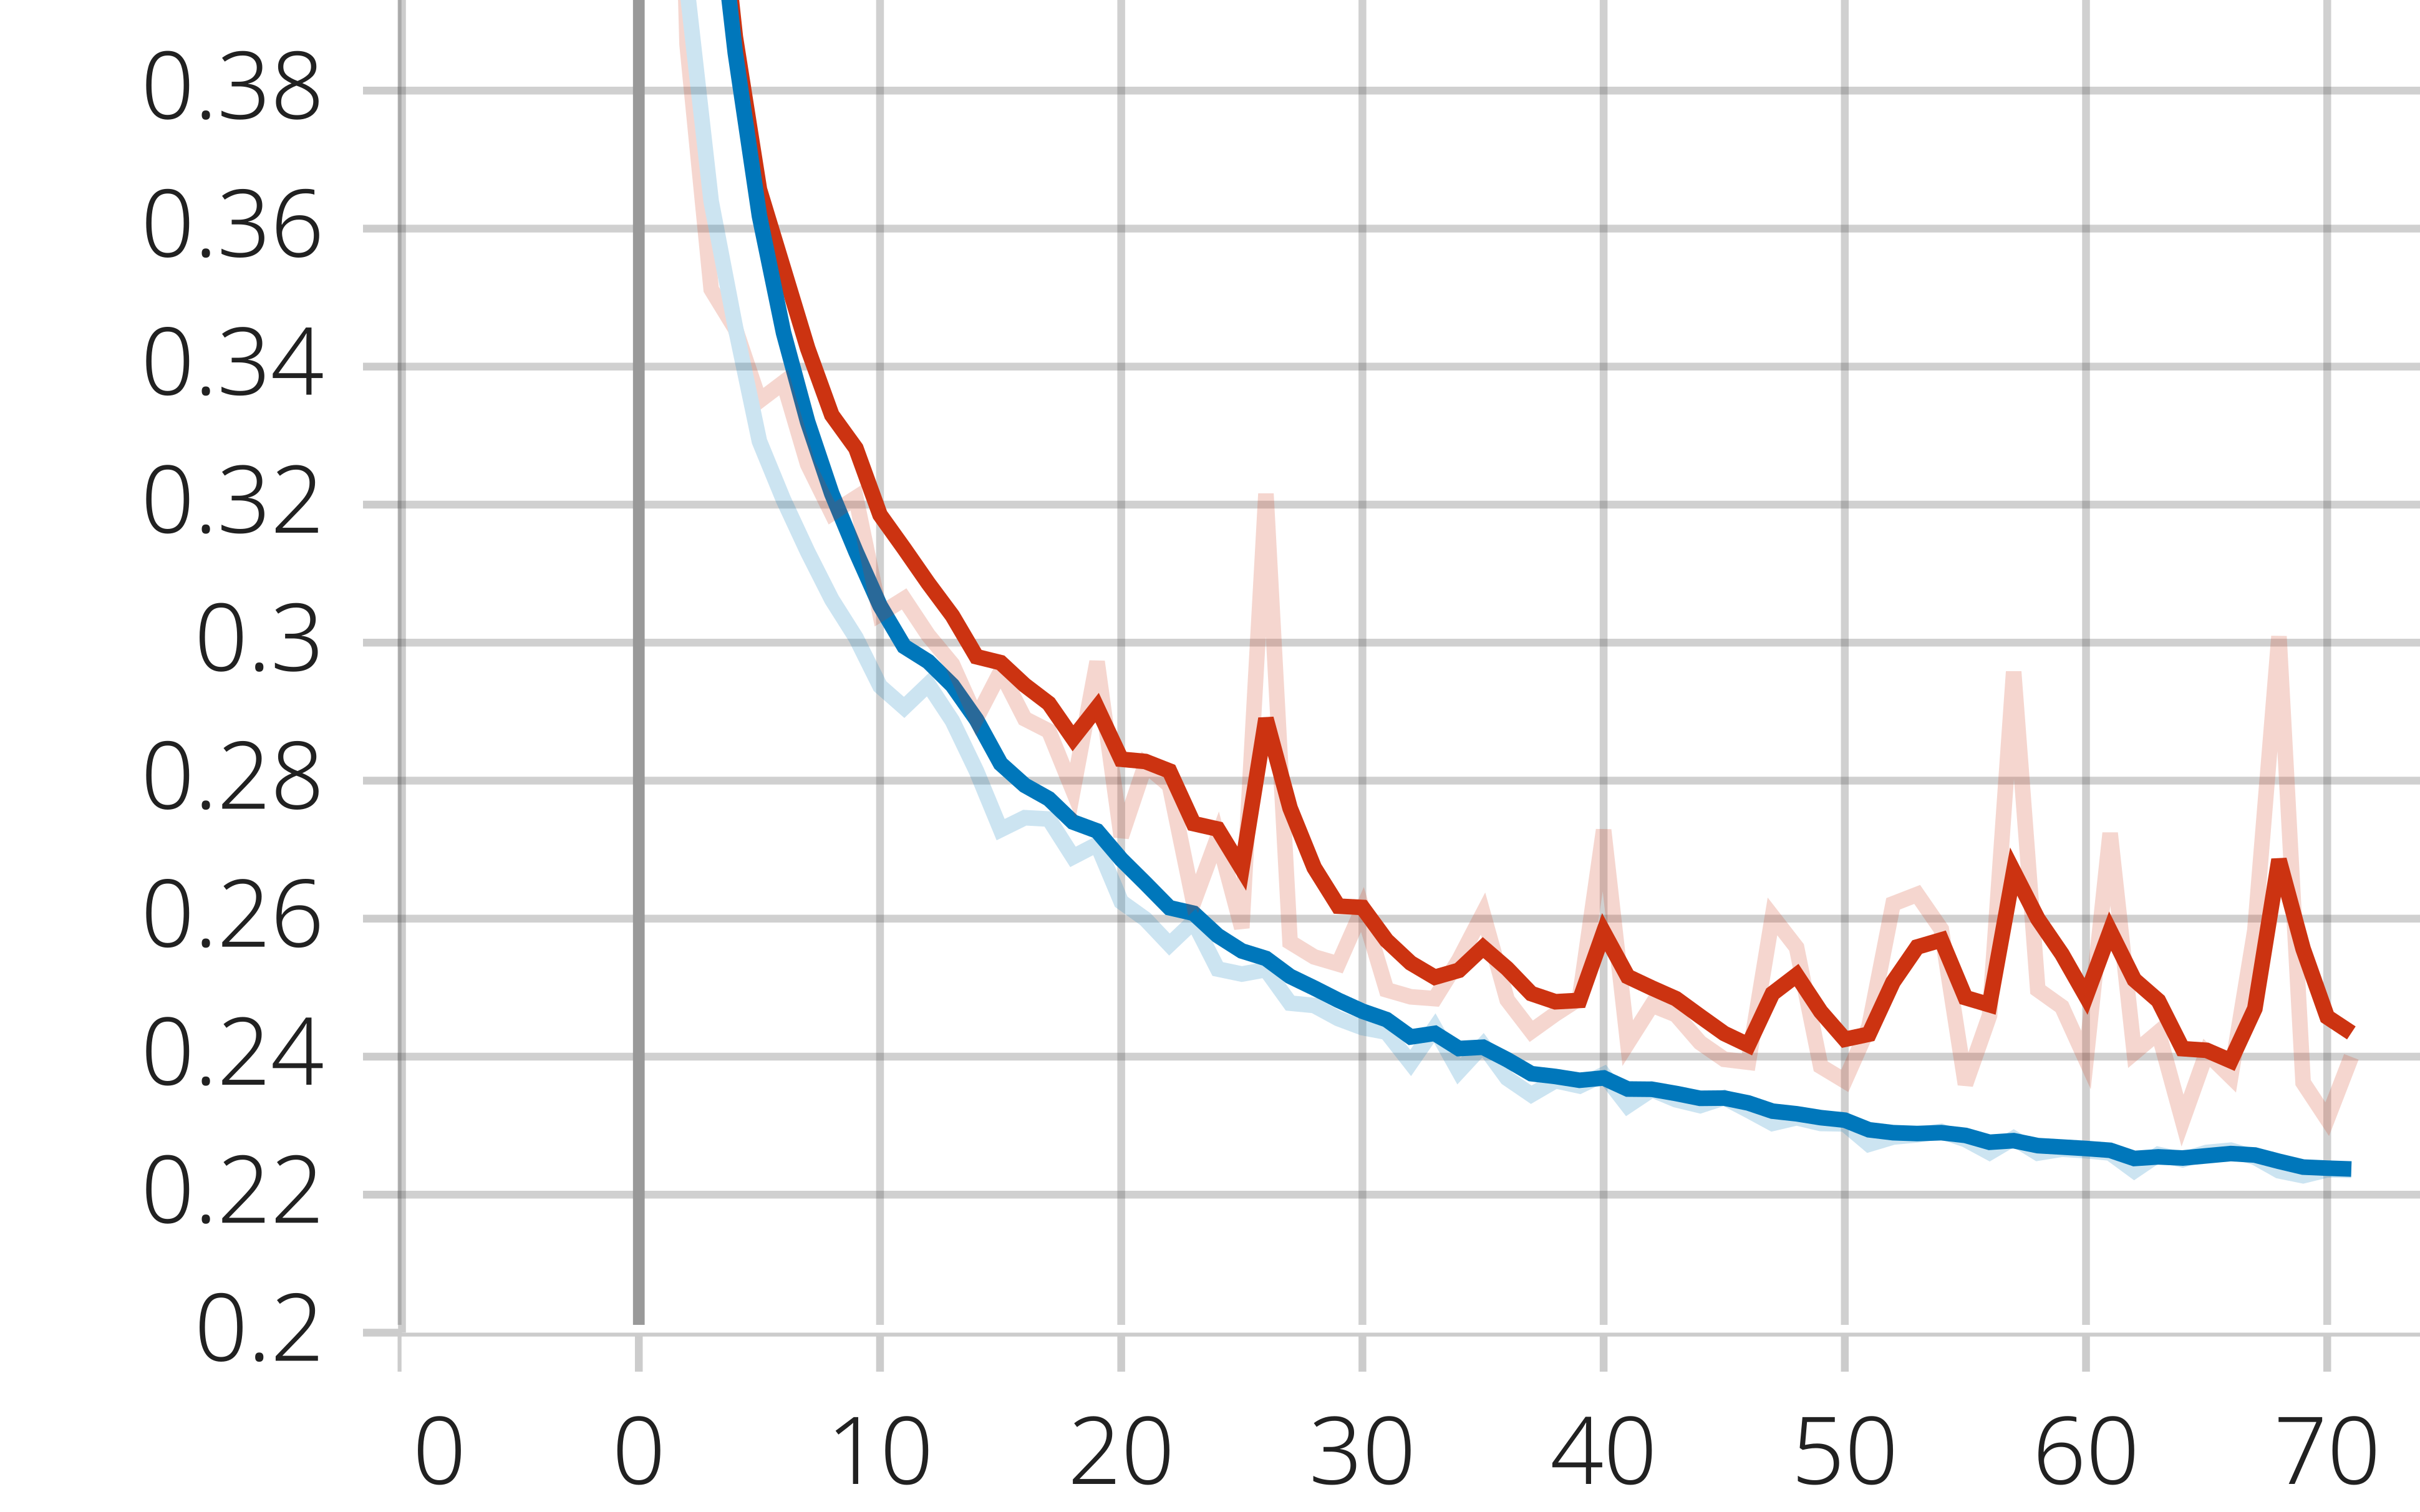
\includegraphics[width=0.24\textwidth]{imgs/Loss_falinxgb.png}
    }
    
    \vspace{0.3cm}
    
    % --- LINHA 3: MobileNetV2 ---
    \subfloat[MobileNetV2: Accuracy \label{fig:wafer_acc_mobiv2}]{
        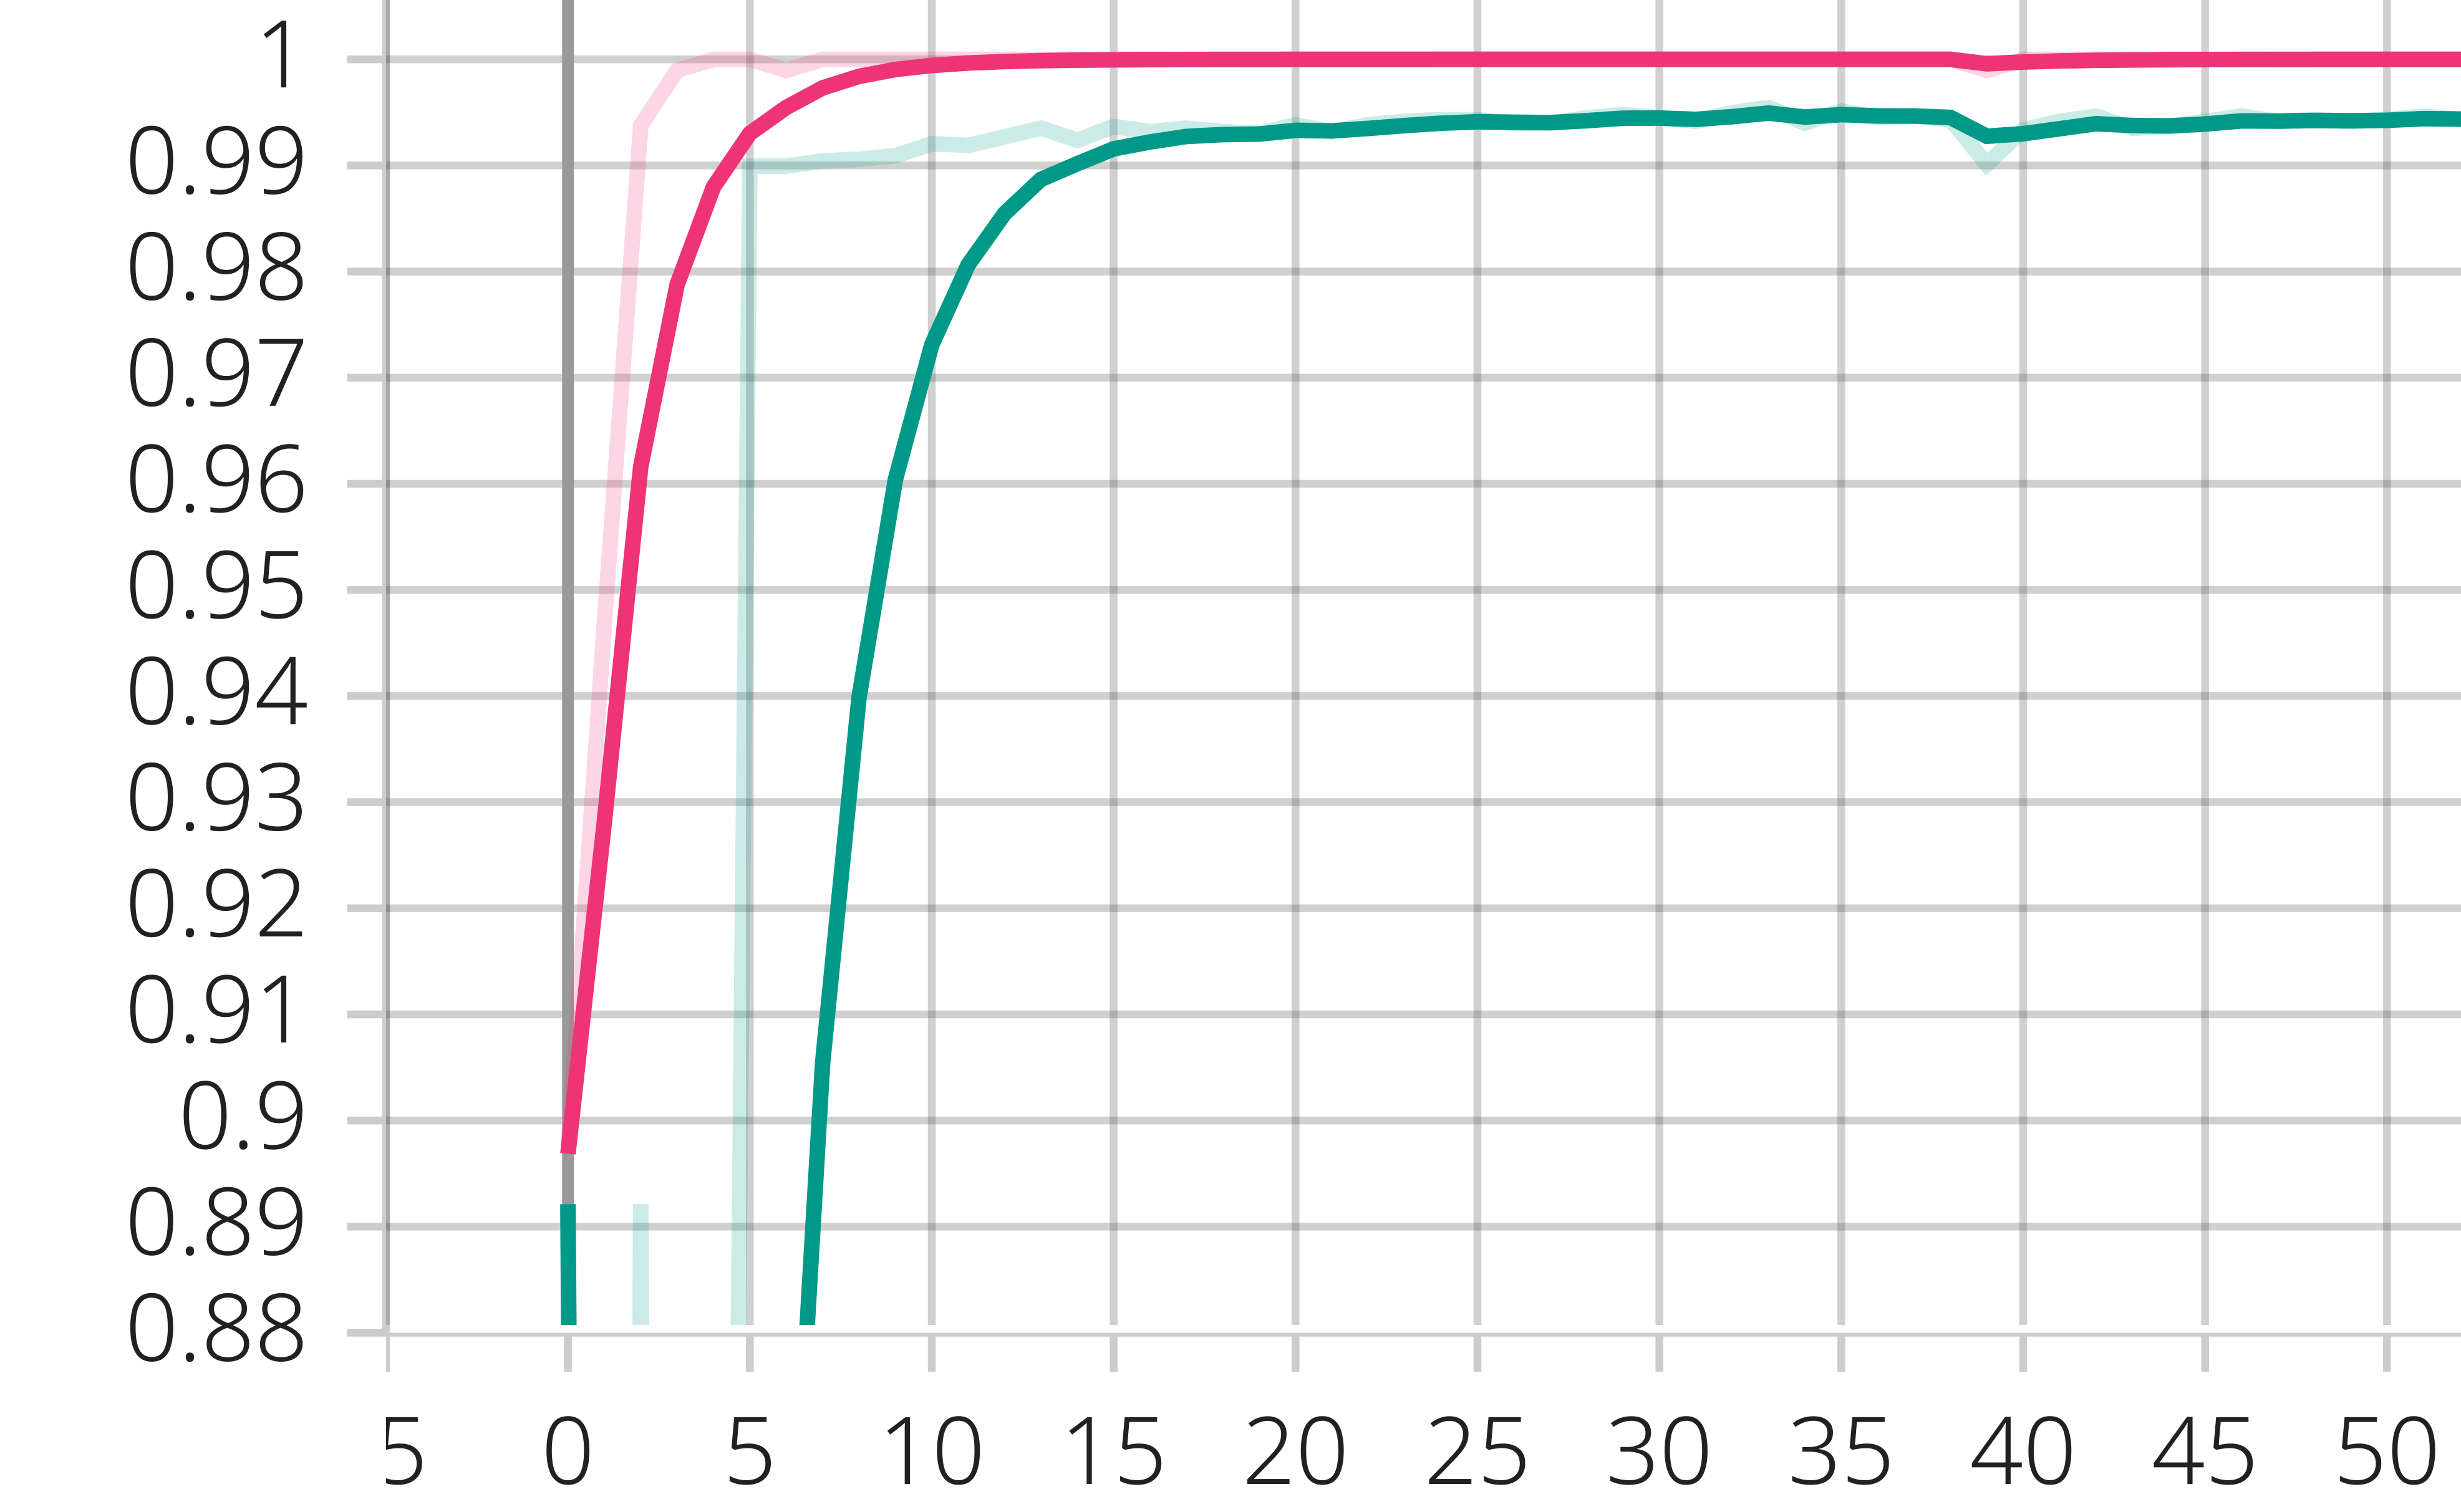
\includegraphics[width=0.24\textwidth]{imgs/Accuracy_mobiv2.png}
    }
    % \hfill
    \subfloat[MobileNetV2: Loss \label{fig:wafer_loss_mobiv2}]{
        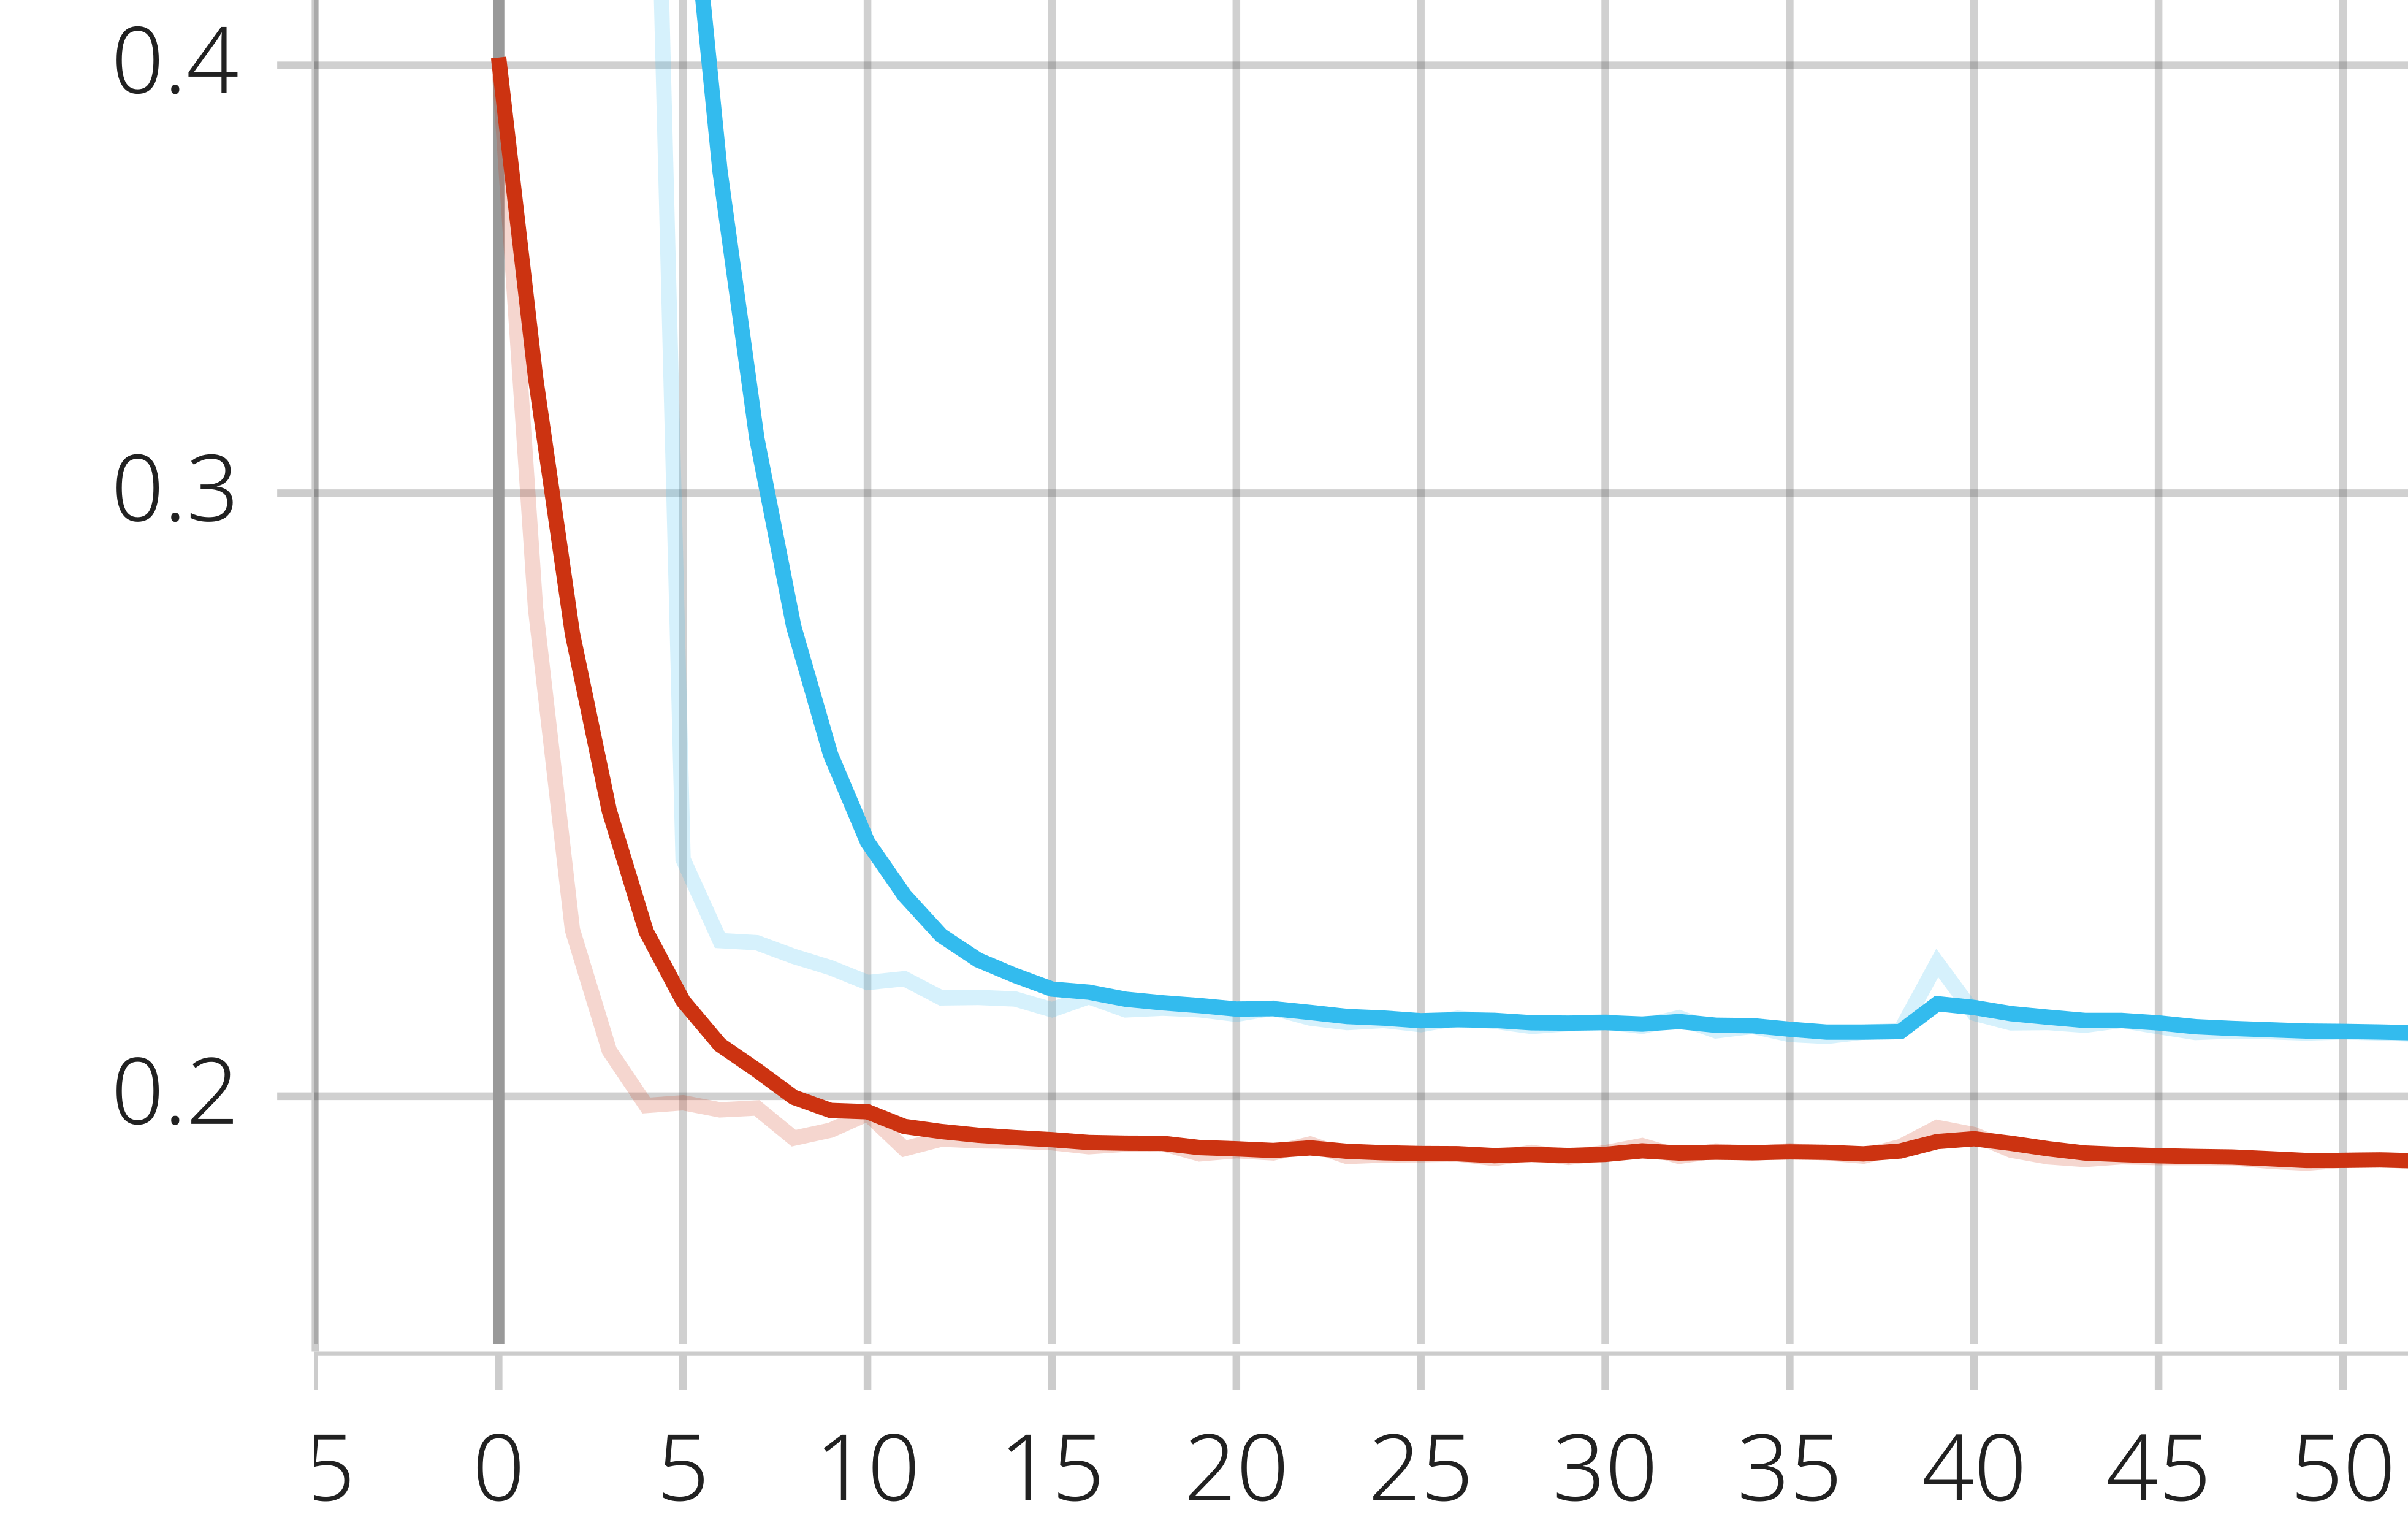
\includegraphics[width=0.24\textwidth]{imgs/Loss_mobiv2.png}
    }
    
    \vspace{0.3cm}
    
    % --- LINHA 4: MobileNet-XGB ---
    \subfloat[MobileNet-XGB: Accuracy \label{fig:wafer_acc_mobixgb}]{
        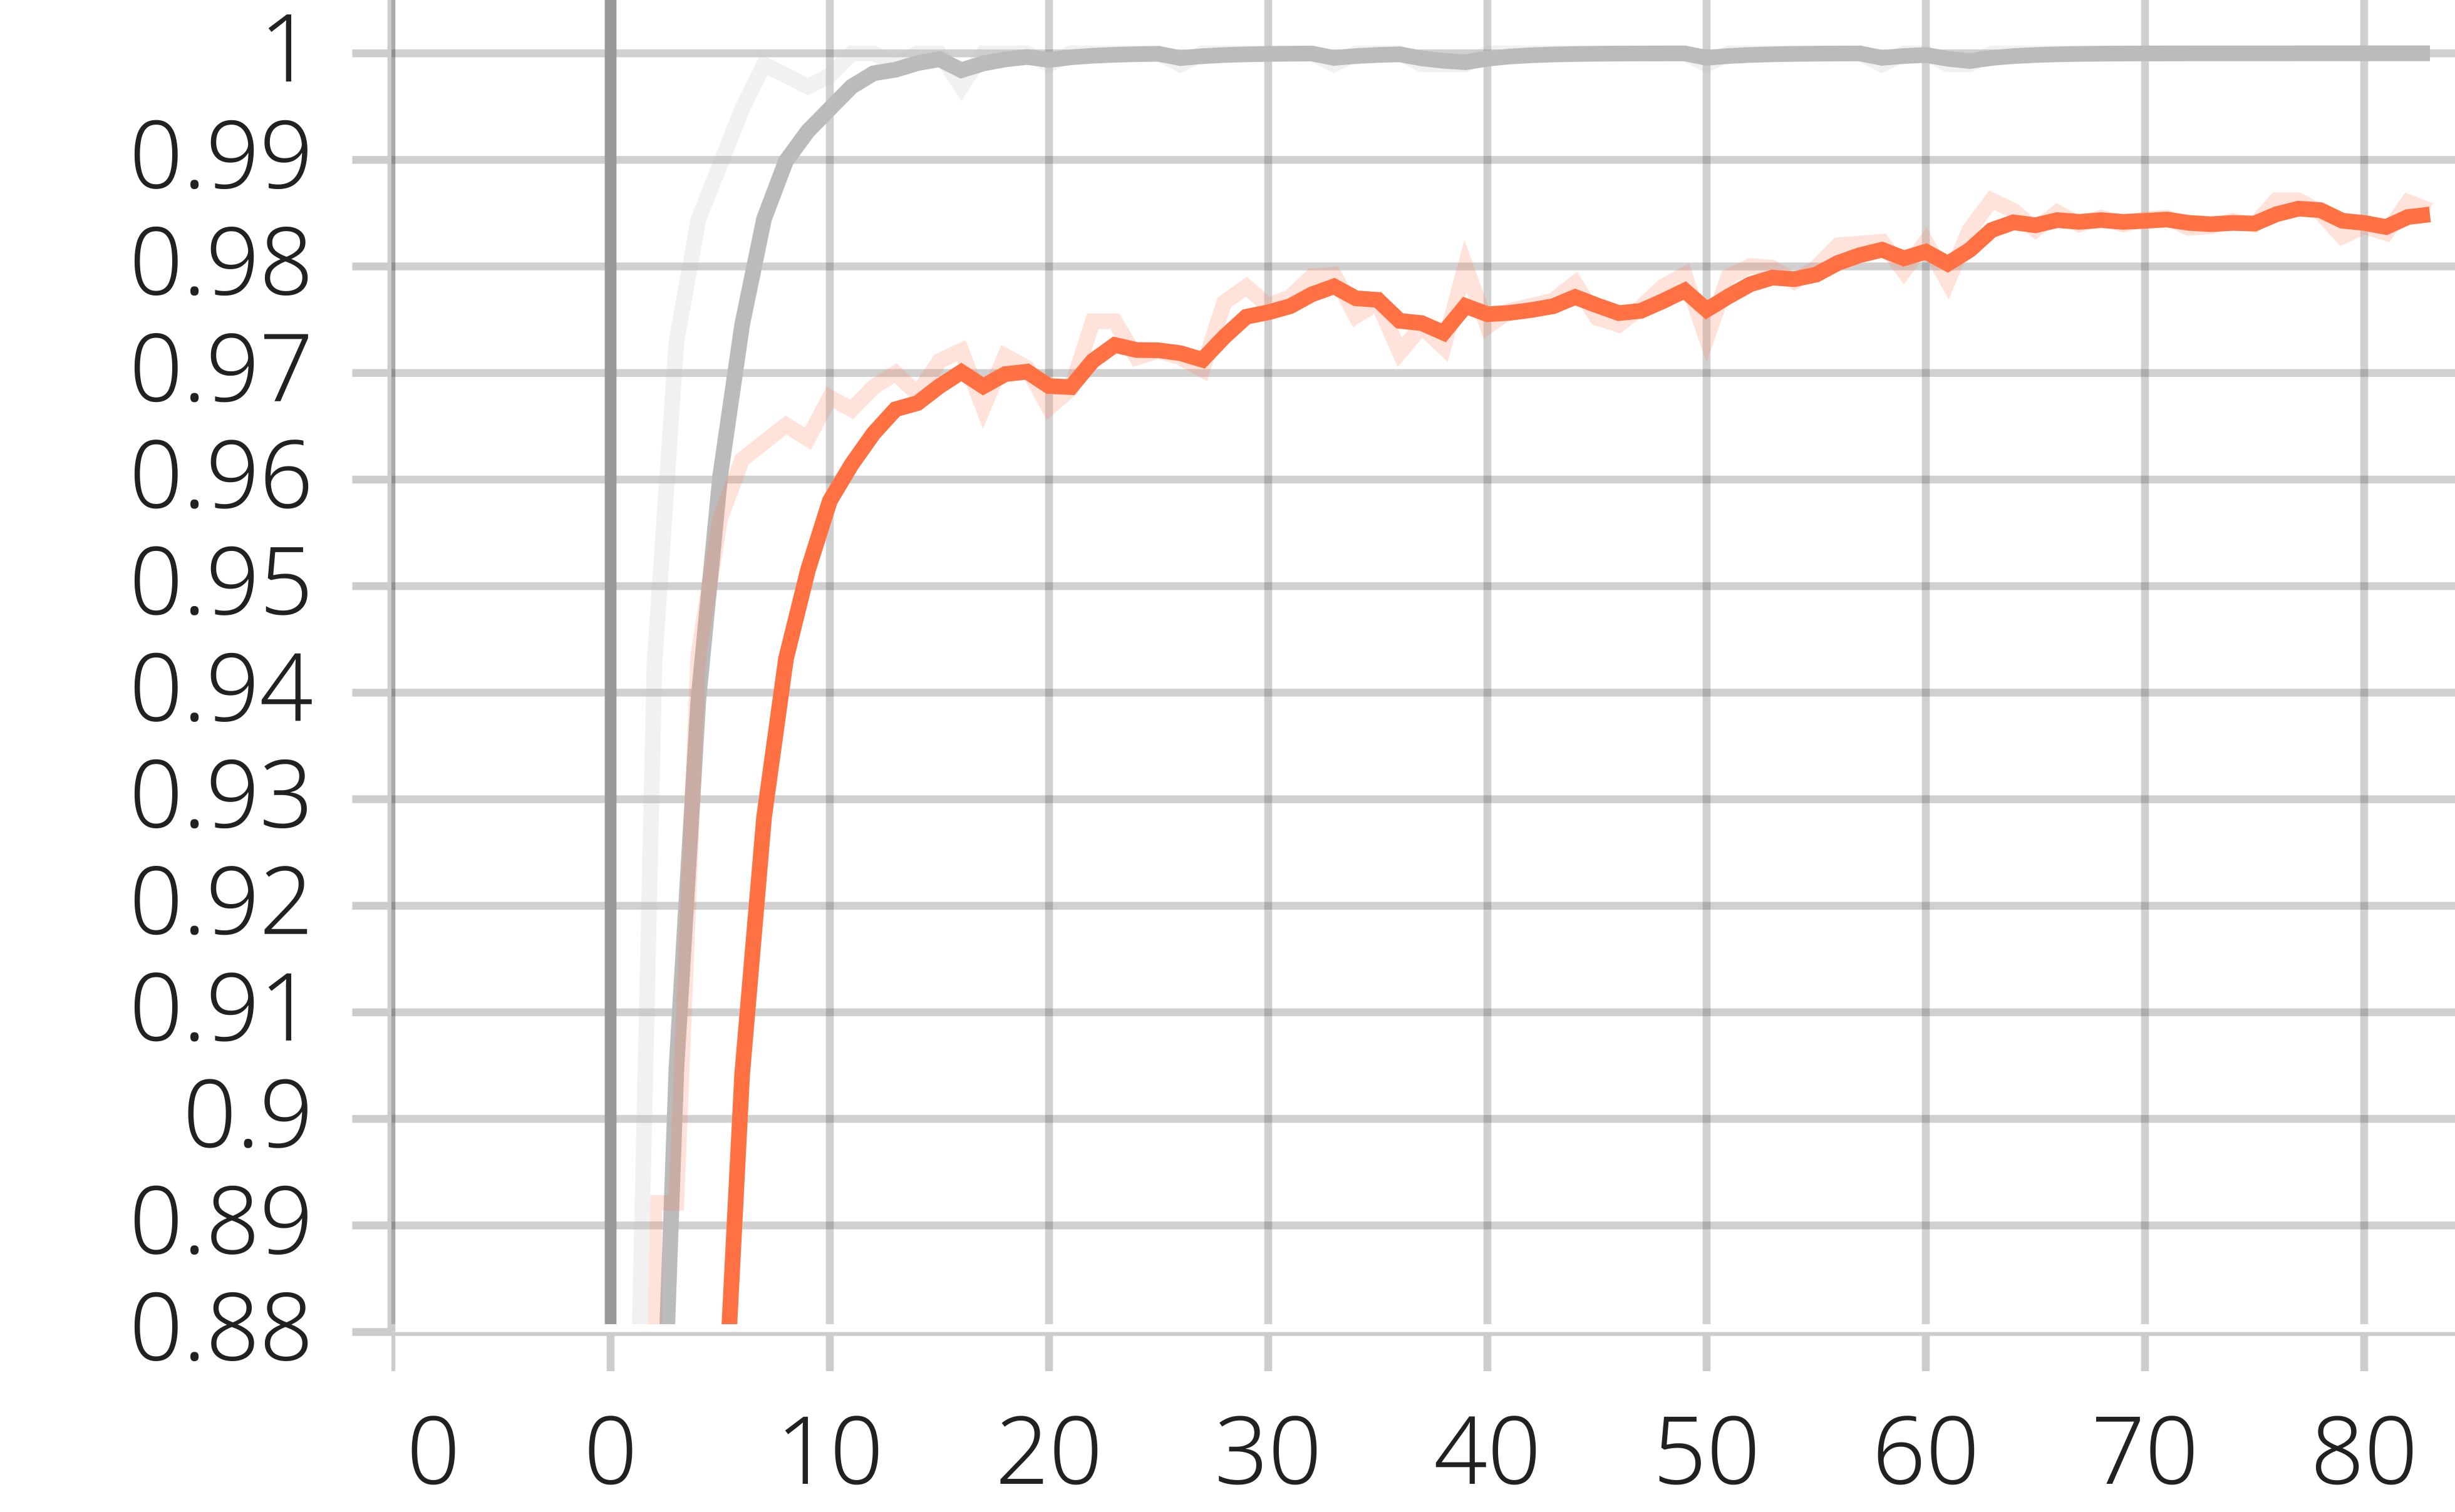
\includegraphics[width=0.24\textwidth]{imgs/Accuracy_mobixgb.png}
    }
    % \hfill
    \subfloat[MobileNet-XGB: Loss \label{fig:wafer_loss_mobixgb}]{
        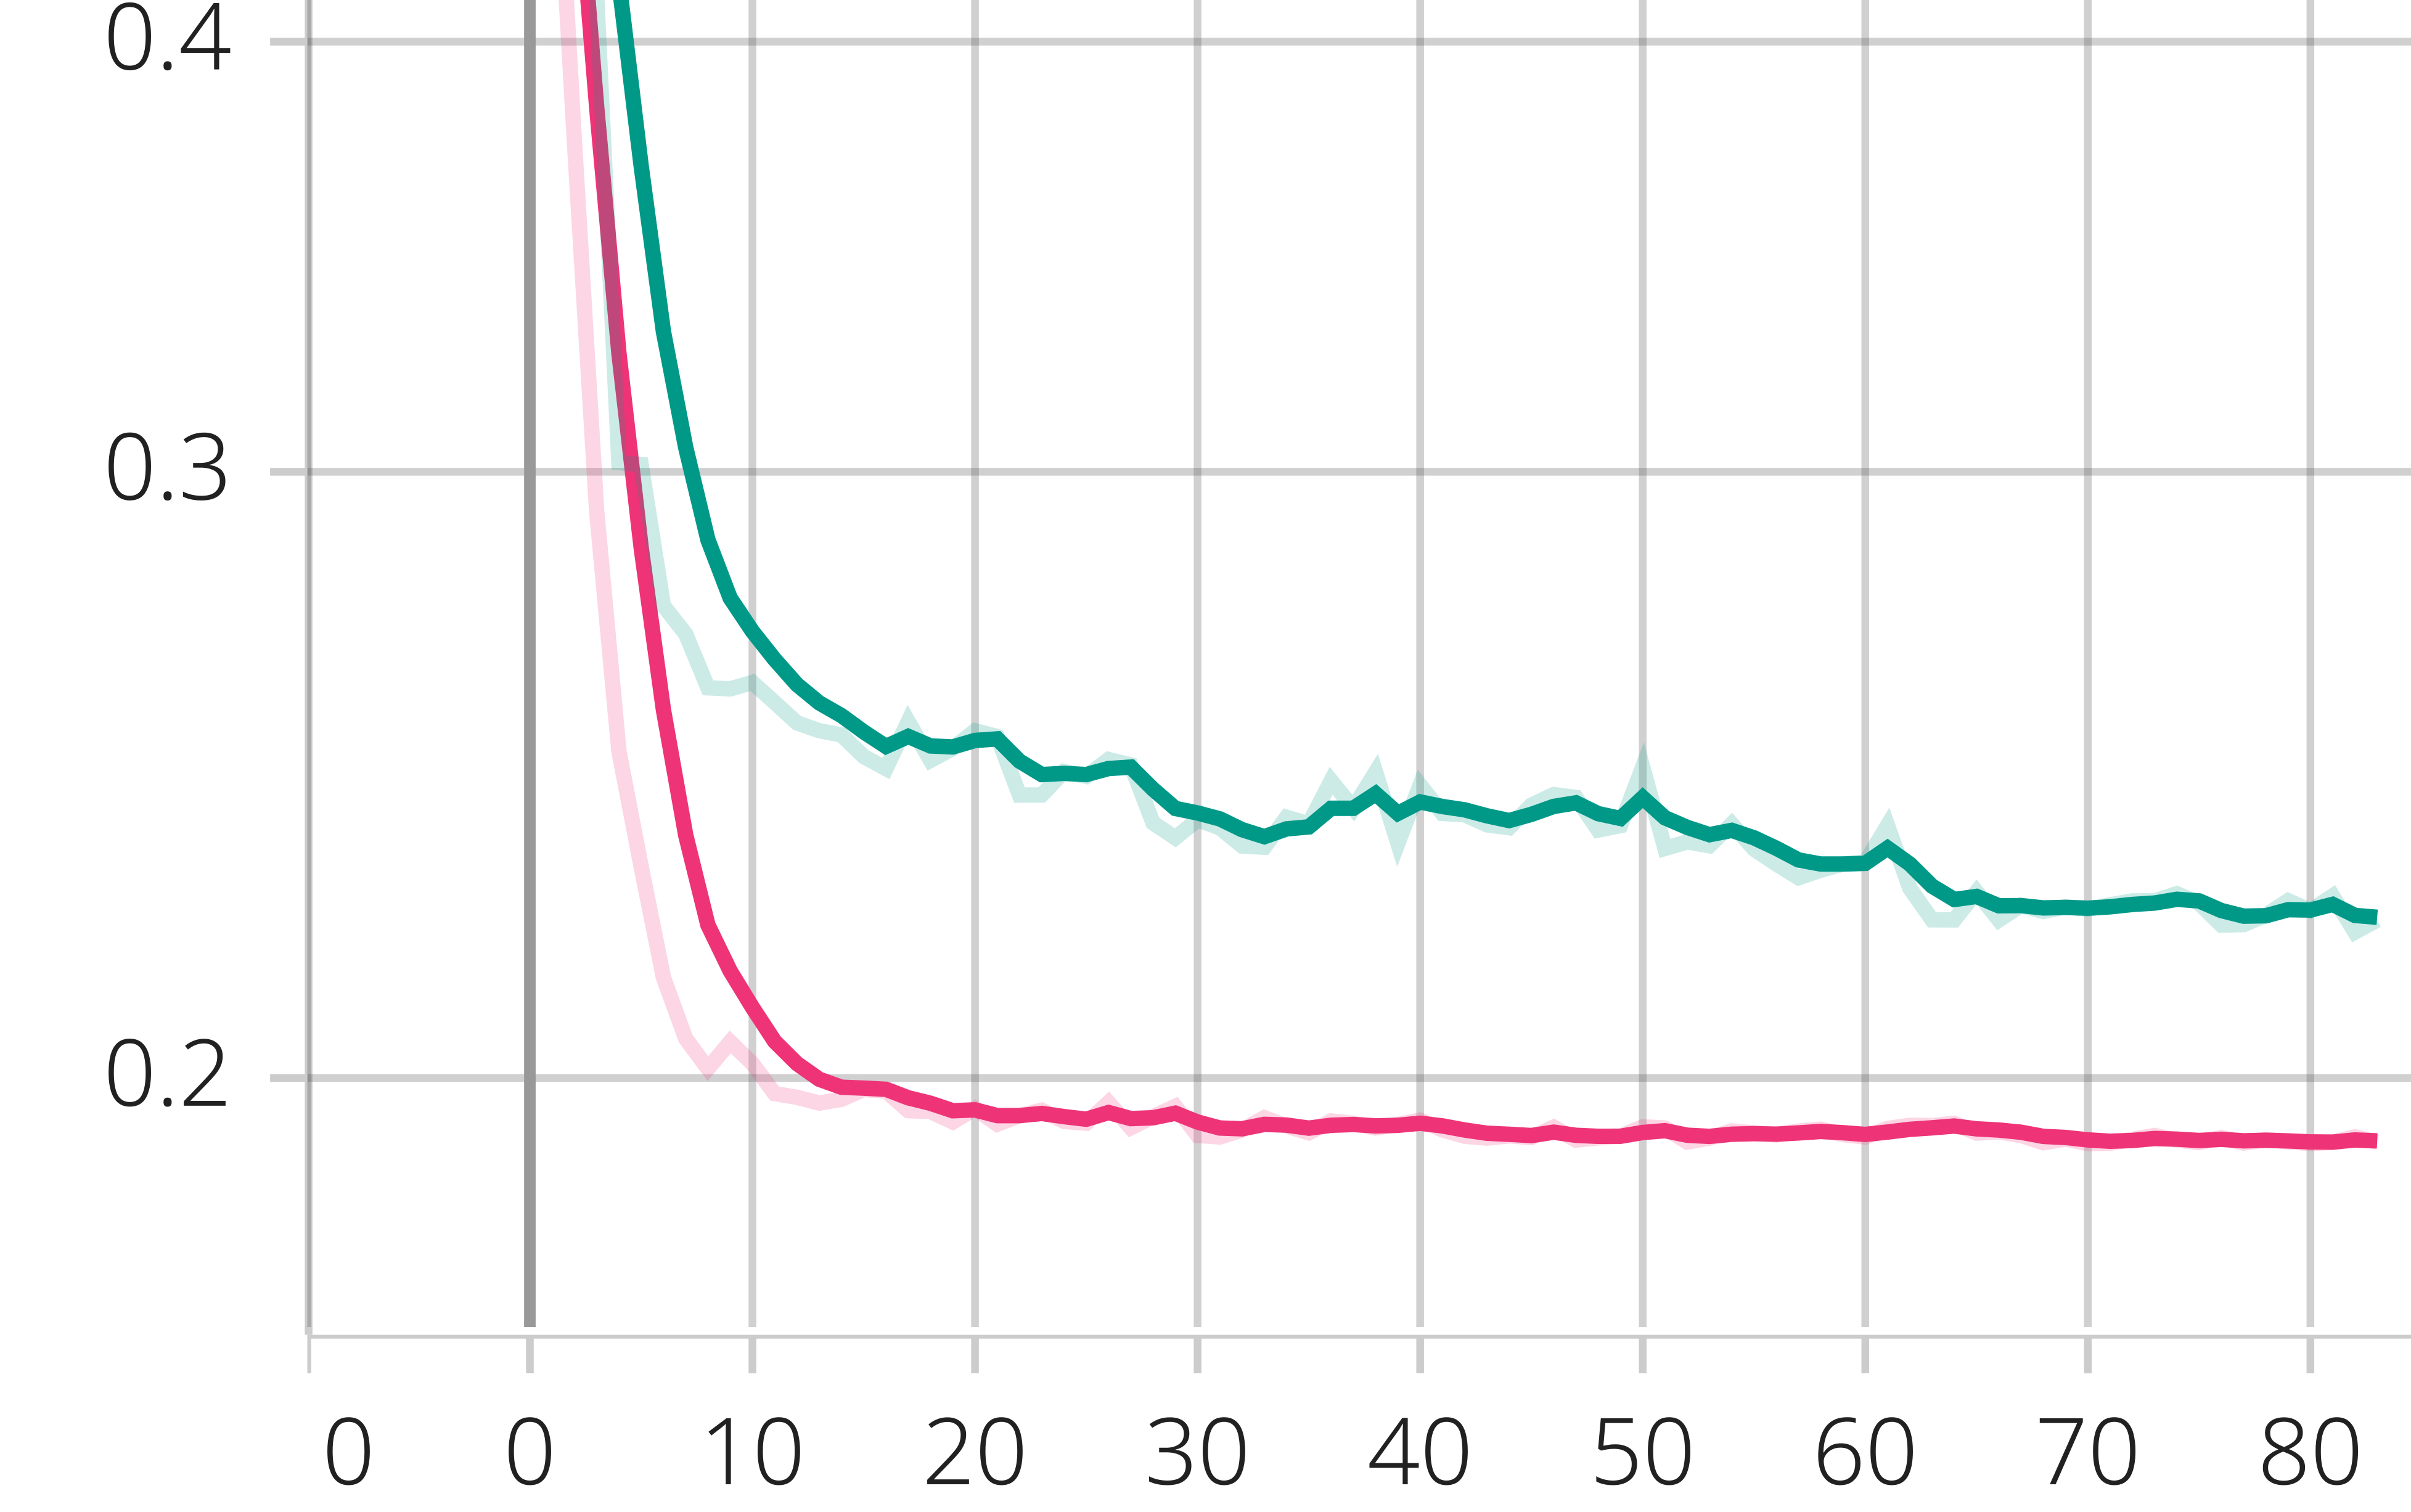
\includegraphics[width=0.24\textwidth]{imgs/Loss_mobixgb.png}
    }
    
    \caption{Training and validation metrics (Accuracy and Loss) for the Wafer dataset across different architectures. The dynamic early-stopping mechanism ensures convergence without severe overfitting despite the dataset constraints.}
    \label{fig:wafer_metrics_grid}
\end{figure}

\subsection{Performance and Accuracy Analysis}
\label{subsec:performance_analysis}

\begin{figure*}[!pht]
  \centering
  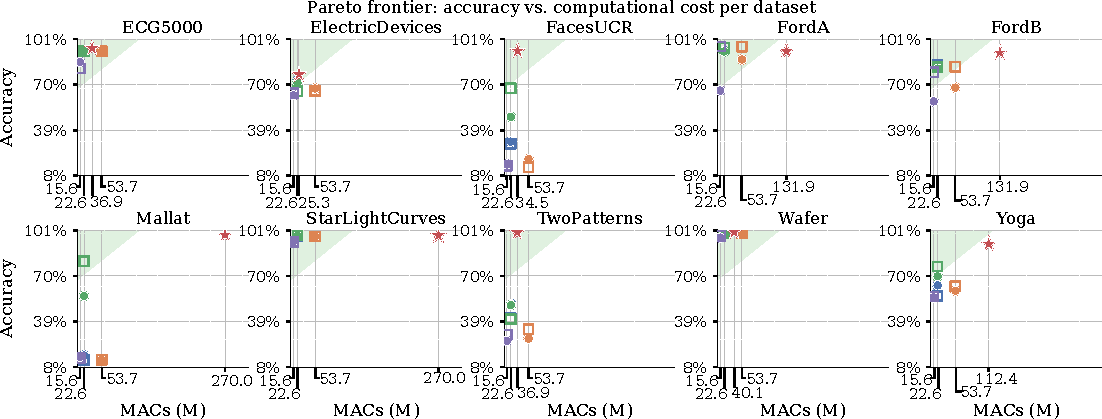
\includegraphics[width=\textwidth]{imgs/fig1_pareto_grid.pdf}
  \caption{Pareto frontier evaluating accuracy versus computational cost per dataset. The markers indicate the model types and their respective Multiplier-Accumulator (MAC) operations: FalinCNN (22.6M MACs) in blue, Falin\_XGB (22.6M MACs) in green, MobileNetV2 (53.7M MACs) in orange, and MobileNet\_XGB (15.6M MACs) in purple. The baseline LSTM-FCN \cite{karim2018lstm} is represented by a red star. Filled markers denote Gramian Angular Fields (GAFS) transformations, while open markers denote Short-Time Fourier Transform (STFS) transformations. The green shaded regions represent the Pareto optimal zones for TinyML compliance.}
  \label{fig:results}
\end{figure*}


The experimental results evaluating the trade-off between classification accuracy and computational cost across the ten selected UCR datasets using both GAFS and STFS representations are illustrated in Fig.~\ref{fig:results}. The grid visualizes the Pareto frontiers for each dataset, highlighting the optimal balance between accuracy (y-axis) and hardware complexity (x-axis, measured in MAC operations).

\subsubsection{Classification Accuracy}
As observed in the dataset-specific plots of Fig.~\ref{fig:results}, the baseline LSTM-FCN model (represented by the red star) consistently achieves high accuracy across most datasets, establishing a strict upper bound. However, the proposed FALIN framework demonstrates highly competitive performance within the TinyML-compliant footprint, frequently landing inside the shaded green Pareto optimal zones, particularly on datasets characterized by strong periodic or spectral components. 
\begin{itemize}
    \item \textbf{High-Performance Scenarios:} For datasets such as \textit{ECG5000}, \textit{Wafer}, and \textit{FordA}, the lightweight configurations track the baseline accuracy very closely (reaching near 100\% in several cases) under both GAFS and STFS transformations. This validates that 1D-to-2D spatial mappings successfully preserve critical discriminative temporal features without requiring heavy sequential models.
    \item \textbf{Impact of the Hybrid Classifier (XGBoost):} The integration of the XGBoost backend yields significant accuracy recoveries in challenging structural datasets. For instance, in the \textit{Mallat} dataset, the standard \textit{FalinCNN} suffers from severe performance degradation (falling near 10\% accuracy); however, the hybrid \textit{Falin\_XGB} architecture recovers a substantial portion of this loss, pushing accuracy above 50\%. A similar upward trend is observed in datasets like \textit{FacesUCR} and \textit{TwoPatterns}, proving that tree-based ensembles operating on lightweight CNN-extracted features provide a much more robust decision boundary than standard linear layers when data scale or structural complexity is an issue.
\end{itemize}

\subsubsection{Hardware Complexity and TinyML Feasibility}
The core advantage of the FALIN framework becomes evident when observing the horizontal axis of the Pareto plots. While the sequential LSTM-FCN baseline achieves high accuracy, it introduces a prohibitive computational burden for resource-constrained edge devices, often positioned far to the right (demanding nearly 270 Million MAC operations per inference for long sequences).

In stark contrast, the proposed architectures maintain an extremely compact and predictable computational footprint. Both \textit{FalinCNN} and \textit{Falin\_XGB} consistently require exactly 22.6 Million MACs, while the \textit{MobileNet\_XGB} variant drops even further to 15.6 Million MACs. This represents an order-of-magnitude reduction in arithmetic complexity compared to the baseline. Furthermore, by shifting the decision head from parameter-heavy fully connected layers to Look-Up-Table (LUT) friendly tree structures in the XGBoost variants, FALIN successfully minimizes on-chip memory access cycles. Falling securely within the green shaded Pareto regions, this trade-off, sacrificing a marginal percentage of accuracy in exchange for a massive reduction in computational load, strongly supports the viability of FALIN for strict, real-time TinyML and FPGA-based edge deployment.

\section{Conclusion}
\label{sec:conclusions}

To evaluate the proposed FALIN framework, experimental analyses were conducted across ten distinct datasets from the UCR Time Series Archive comparing classification accuracy and hardware complexity against state-of-the-art temporal models like LSTM-FCN. As illustrated in Fig.~\ref{fig:results}, the 1D-to-2D spatial mappings using GAF and STFT successfully preserve critical discriminative temporal features, tracking the baseline accuracy perfectly for periodic waveforms such as \textit{ECG5000} and \textit{Wafer}. Crucially, the integration of the hybrid XGBoost classifier  delivers robust decision boundaries that recover catastrophic accuracy drops experienced by standard linear layers in structurally complex datasets, notably achieving a substantial accuracy rebound in the \textit{Mallat} and \textit{FacesUCR} benchmarks. From a hardware perspective, while the sequential LSTM-FCN baseline demands a prohibitive computational burden exceeding 250 Million MACs for long-sequence inputs, the FALIN framework consistently squashes the arithmetic overhead to well below 25 Million MACs across all datasets. This order-of-magnitude reduction in MAC, coupled with LUT-friendly tree ensemble execution, demonstrates an optimized accuracy-to-MAC efficiency that bypasses physical memory bottlenecks. Consequently, FALIN achieves a highly compact, TinyML-compliant footprint, validating its strict feasibility for real-time, FPGA-based edge computing deployment where physical resources are heavily constrained.


% --- Bibliography ---
\bibliographystyle{IEEEtran}
\bibliography{reference}

\end{document}